\documentclass[aspectratio=169]{beamer}
\usetheme{metropolis}  

\metroset{block=fill}

\setlength{\parindent}{0pt}
\usepackage[utf8]{inputenc}
\usepackage{amsbsy}
\usepackage{amsmath}
\usepackage{enumitem}
\usepackage{hyperref}
\usepackage{array}
\usepackage[T1]{fontenc}
\usepackage{tikz}
\usepackage{latexsym,xcolor,multicol,booktabs,calligra}
\usepackage{amsmath,amssymb,BOONDOX-cal,bm}	
\usepackage{graphicx,stackengine}   
\usepackage{xcolor}
\usepackage[sfdefault]{AlegreyaSans}
\usepackage{tabularx} 

\definecolor{white}{RGB}{255,255,255}
\setbeamercolor{background canvas}{bg=white}
\setbeamercolor{normal text}{bg=white}

\title{Causal Inference Project:\\ Impact of Scholarships on Student Success}
\date{April 04th, 2025}
\author{Anushka Mukherjee, Lucie Marimar, Jort Koks, Jakob Sarrazin}
\institute{Machine Learning for Econometrics \\ ENSAE, IP Paris \\ Bruno Crépon, Matthieu Doutreligne}

% ---------------------------------------
% Begin Document
% ---------------------------------------

\begin{document}
  \maketitle
  
% ---------------------------------------
% Section Motivation
% ---------------------------------------

   \section{1. Motivation}
  
  \begin{frame}{Motivation I}
  		\begin{columns}
	\begin{column}{0.7\textwidth}
	\textbf{Retention and Completion: A Core Challenge for Universities}

  		\begin{itemize}
  		\item [$\rightarrow$] \textbf{High dropout rates} are a persistent issue in higher education, especially during the first years of study.
  		\item [$\rightarrow$] \textbf{Timely graduation} is crucial for both students (career entry) and universities (funding, reputation
  		\item [$\Rightarrow$] \textbf{Financial constraints} are a major barrier to academic success — especially for socio-economically disadvantaged students.
  	\end{itemize}
  \end{column}

	\begin{column}{0.3\textwidth}
	\begin{center}
     
\includegraphics[width=1\textwidth]{Tex_Pictures/hat.png}
     \end{center}
	\end{column}

\end{columns}

  	
  \end{frame}
  
  \begin{frame}{Motivation II}
  	\textbf{Scholarships as a Tool to Improve Student Retention and Graduation}
  	
  	\begin{itemize}
  		\item [$\rightarrow$]  \textbf{Scholarship programs} are widely used as an intervention, but:
  		\begin{itemize}
  		  		\item [--] Their  \textbf{causal effect} on student outcomes is difficult to measure
  		  		\item [--] Many studies show correlations, but few rigorously identify causality.
   		\end{itemize}
   		\item [$\rightarrow$] This study uses a \textbf{causal machine learning framework (DML)} to estimate the  \textbf{true effect of scholarships}, adjusting for observed confounders.
   		\item [$\rightarrow$] Findings can inform \textbf{policy decisions} on financial aid allocation and \textbf{targeting of support} for at-risk students.
  	\end{itemize}
  \end{frame}
  
% ---------------------------------------
% Section PICO & RQ
% ---------------------------------------
  
 \section{2. Research Question \& PICO}
  
    \begin{frame}{Research Question}
    \begin{alertblock}{RQ1}
	Does receiving a scholarship \textbf{reduce} the likelihood of \textbf{dropping out} within 3 years?
\end{alertblock}
\vspace{10pt}
    \begin{alertblock}{RQ2}
	Does receiving a scholarship \textbf{increase} the likelihood of \textbf{graduating} within 3 years?
\end{alertblock}
  \end{frame}
  
  \begin{frame}{PICO Formulation}
  \textbf{Population, Intervention, Comparison, Outcome}
  	\begin{itemize}
  		\item [\textbf{P} - ] Undergraduate students at a Portuguese university (N = 4,424), with data on \textit{demographics, socio-economic background, and prior academic performance}.
  		\item [\textbf{I} - ] Receiving a \underline{scholarship} during university studies.
  		\item [\textbf{C} - ] Students without scholarships adjusted for observed covariates \textit{(grades, family background, gender, etc.)}.
  		\item [\textbf{O} - ] Two \underline{binary outcomes} observed 3 years after enrollment:
  
  	\begin{itemize}
  		\item [1.] Dropout vs. Enrolled/Graduated
  		\item [2.] Graduated vs. Dropout/Enrolled
  	\end{itemize}
  	
  	\end{itemize}
  \end{frame}
  

\section{3. Data Overview and Exploratory Analysis}

\begin{frame}{The Dataset}
\vspace{5pt}
\raggedright
\begin{tabular}{ll}
\textbf{Source:} & UC Irvine Machine Learning Repository \\
\textbf{Scope:}  & Administrative records from a Portuguese university \\
                & $\rightarrow$ 4,424 undergraduate students \\
                & $\rightarrow$ Students tracked 3 years after enrollment. \\
\end{tabular}
\begin{center}
\vspace{5pt}
\renewcommand{\arraystretch}{1.2}
\begin{tabularx}{\textwidth}{X | X | X}
\textbf{Outcome Variable} & \textbf{Treatment Variable} & \textbf{Covariates}  (Pre-Treatment)\\[0.5ex]
\hline \hline 
Student status after 3 years: 
\parbox[t]{4cm}{\vspace{-12pt} \begin{itemize}[label=--,leftmargin=1.2em,itemsep=1pt,topsep=2pt]
    \item Dropout
    \item Still enrolled
    \item Graduated
    \item[$\rightarrow$] \textit{Re-coded into two binary variables for RQ1 \& RQ2}
\end{itemize}} &

Received scholarship or not (\textit{Binary variable}) 

& \vspace{-27pt}
\parbox[t]{4cm}{\begin{itemize}[label=--,leftmargin=1.2em,itemsep=1pt,topsep=2pt]
    \item Academic performance before university
    \item Family background
    \item Economic context
    \item Demographics
\end{itemize}}

\end{tabularx}

\end{center}
\end{frame}


\begin{frame}{Outcome Variable}
	\begin{center}
     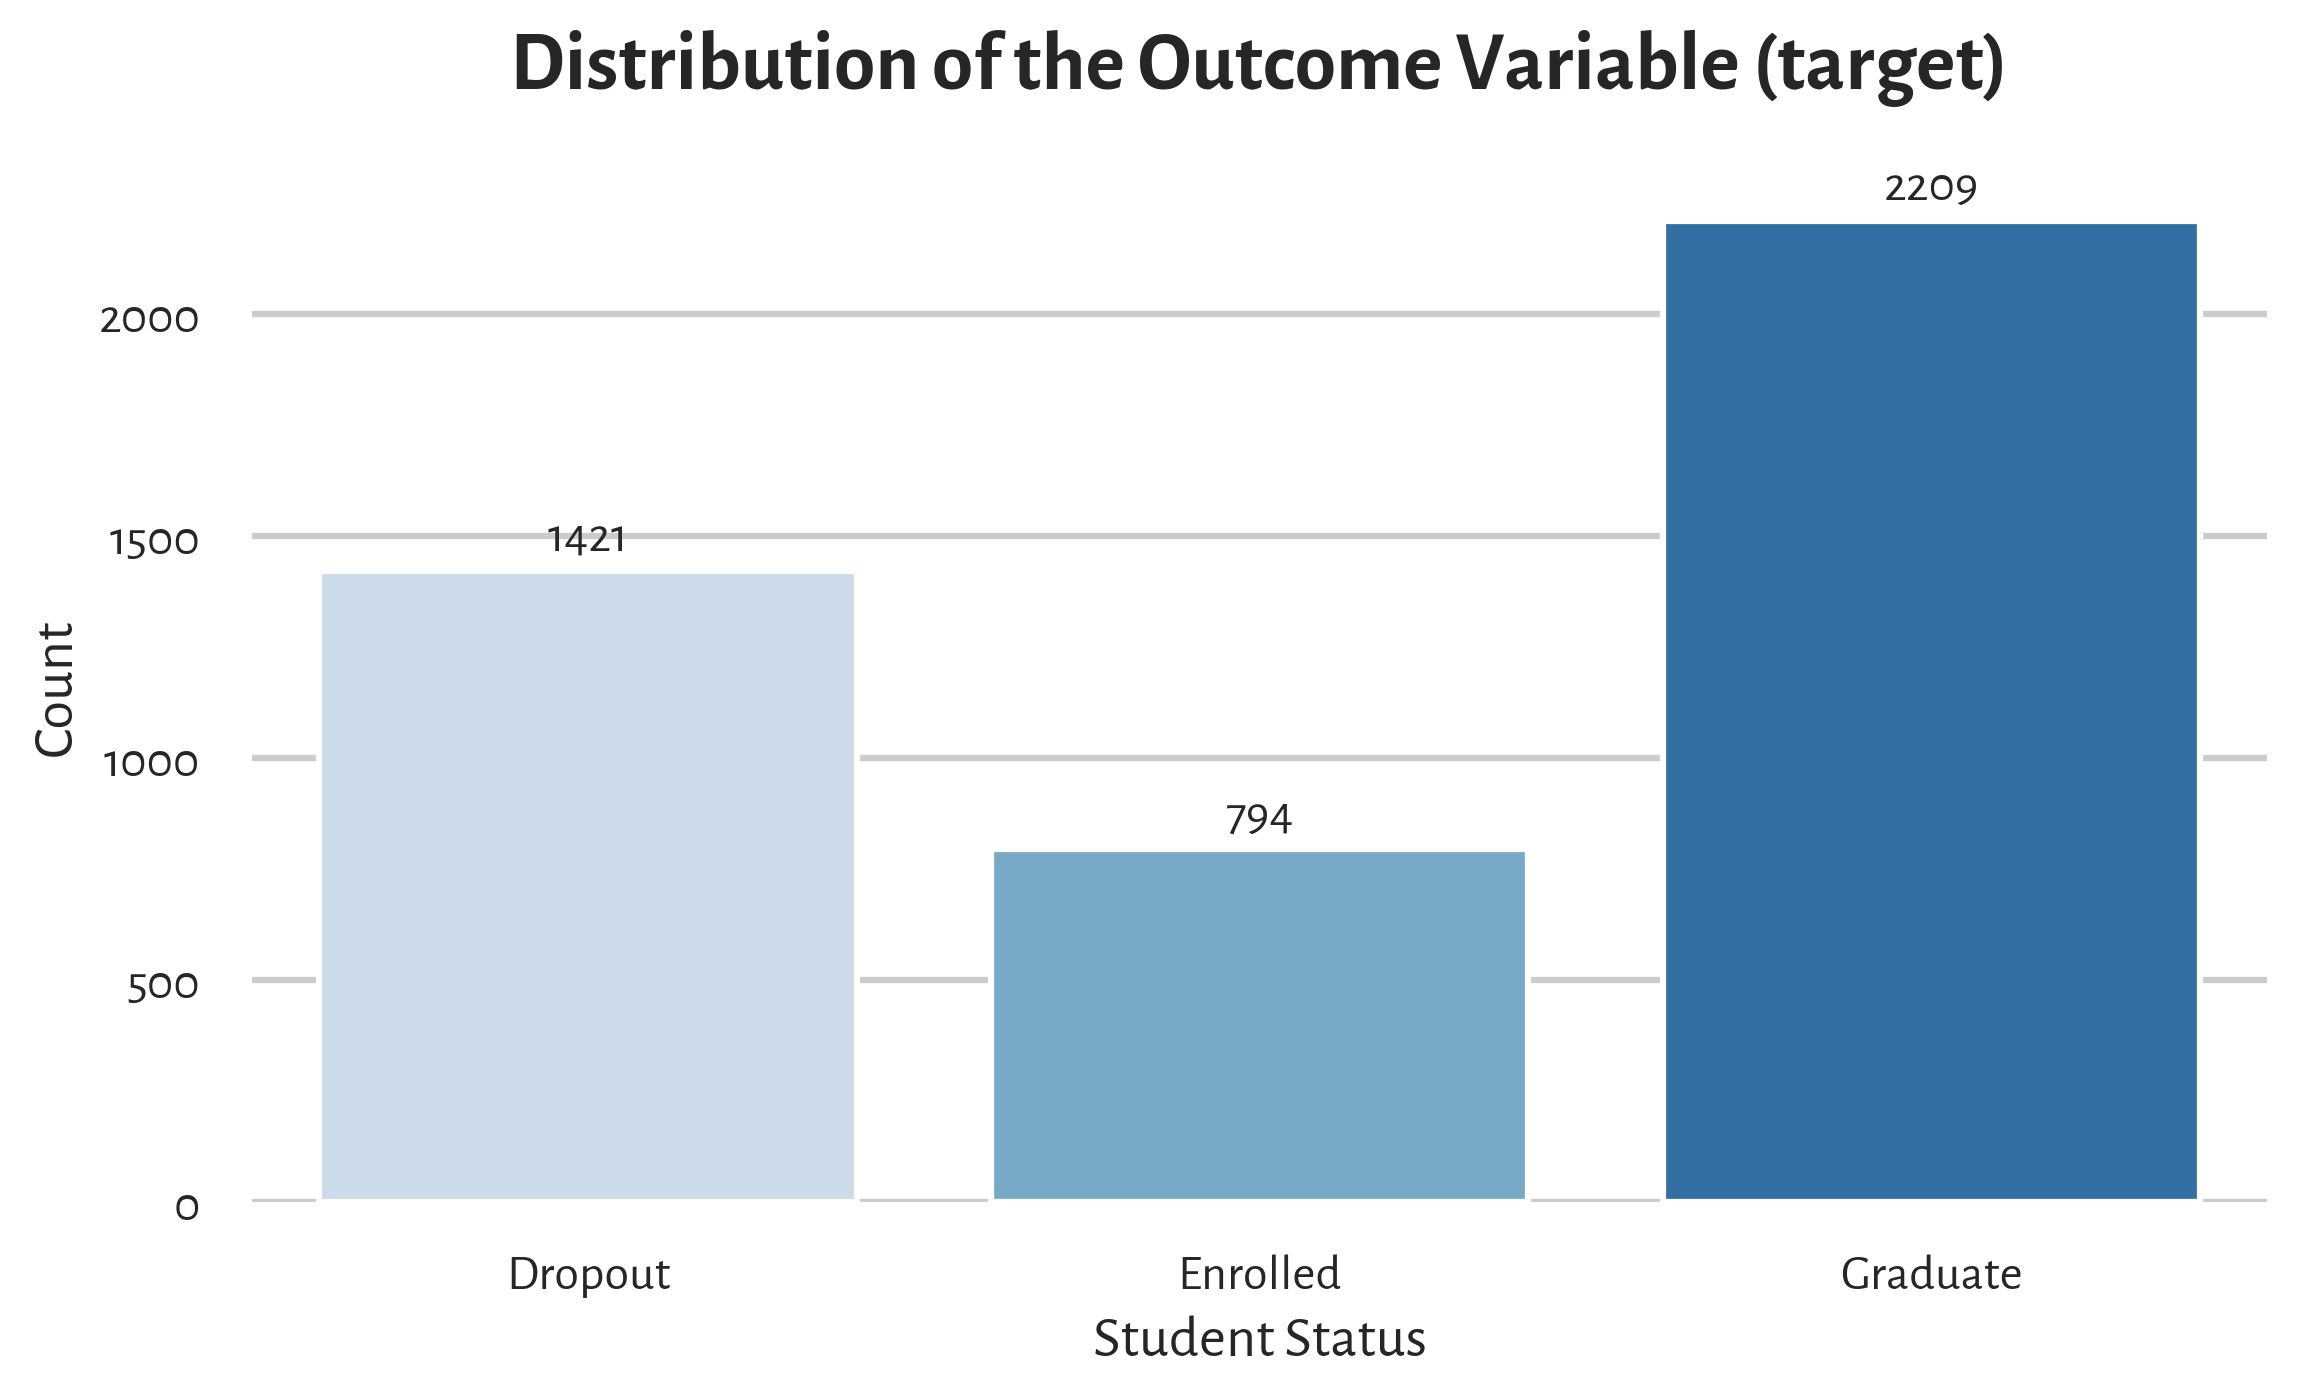
\includegraphics[width=0.85\textwidth]{Tex_Pictures/Graph1.png}
     \end{center}
\end{frame}

\begin{frame}{Treatment vs Outcome Variable}
	\begin{center}
     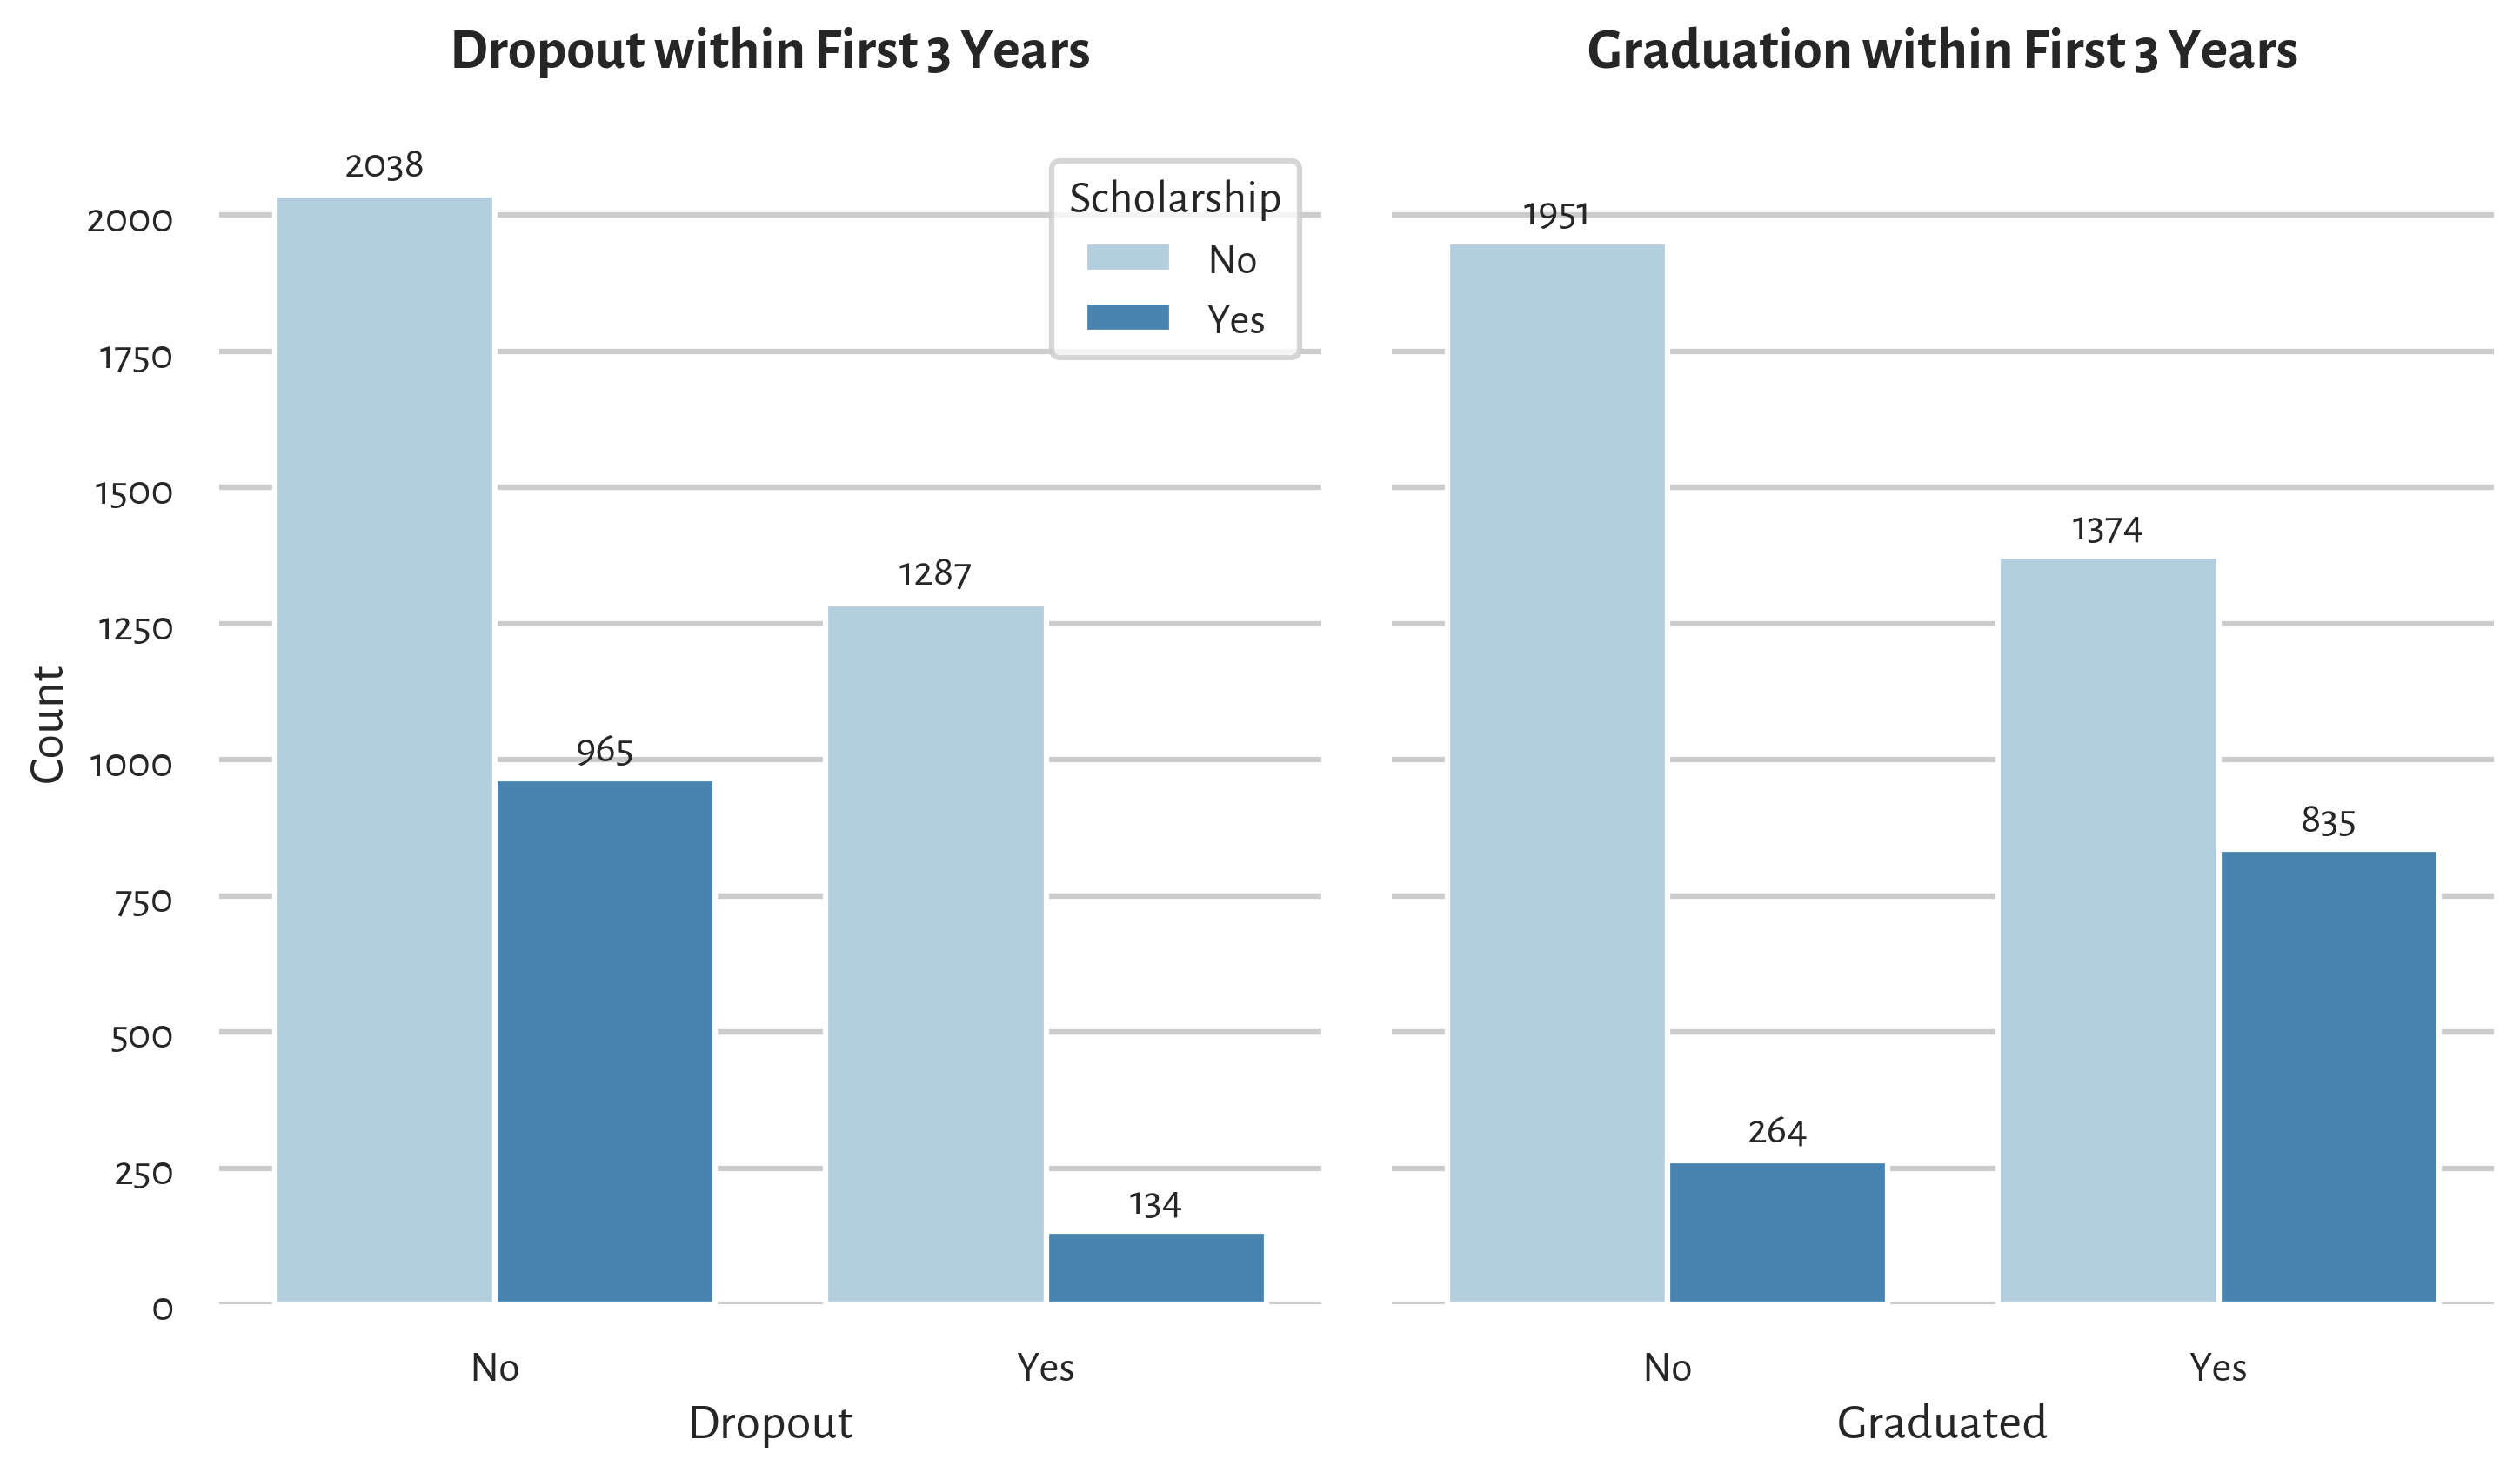
\includegraphics[width=0.8\textwidth]{Tex_Pictures/Graph2.png} \\
     \small
     Dropout (Graduation) probability decreases (increases) by 68.50\% (83.86\%) for scholarship holders.
     \end{center}
\end{frame}

\begin{frame}{Covariates: Academic Preperation}
	\begin{center}
     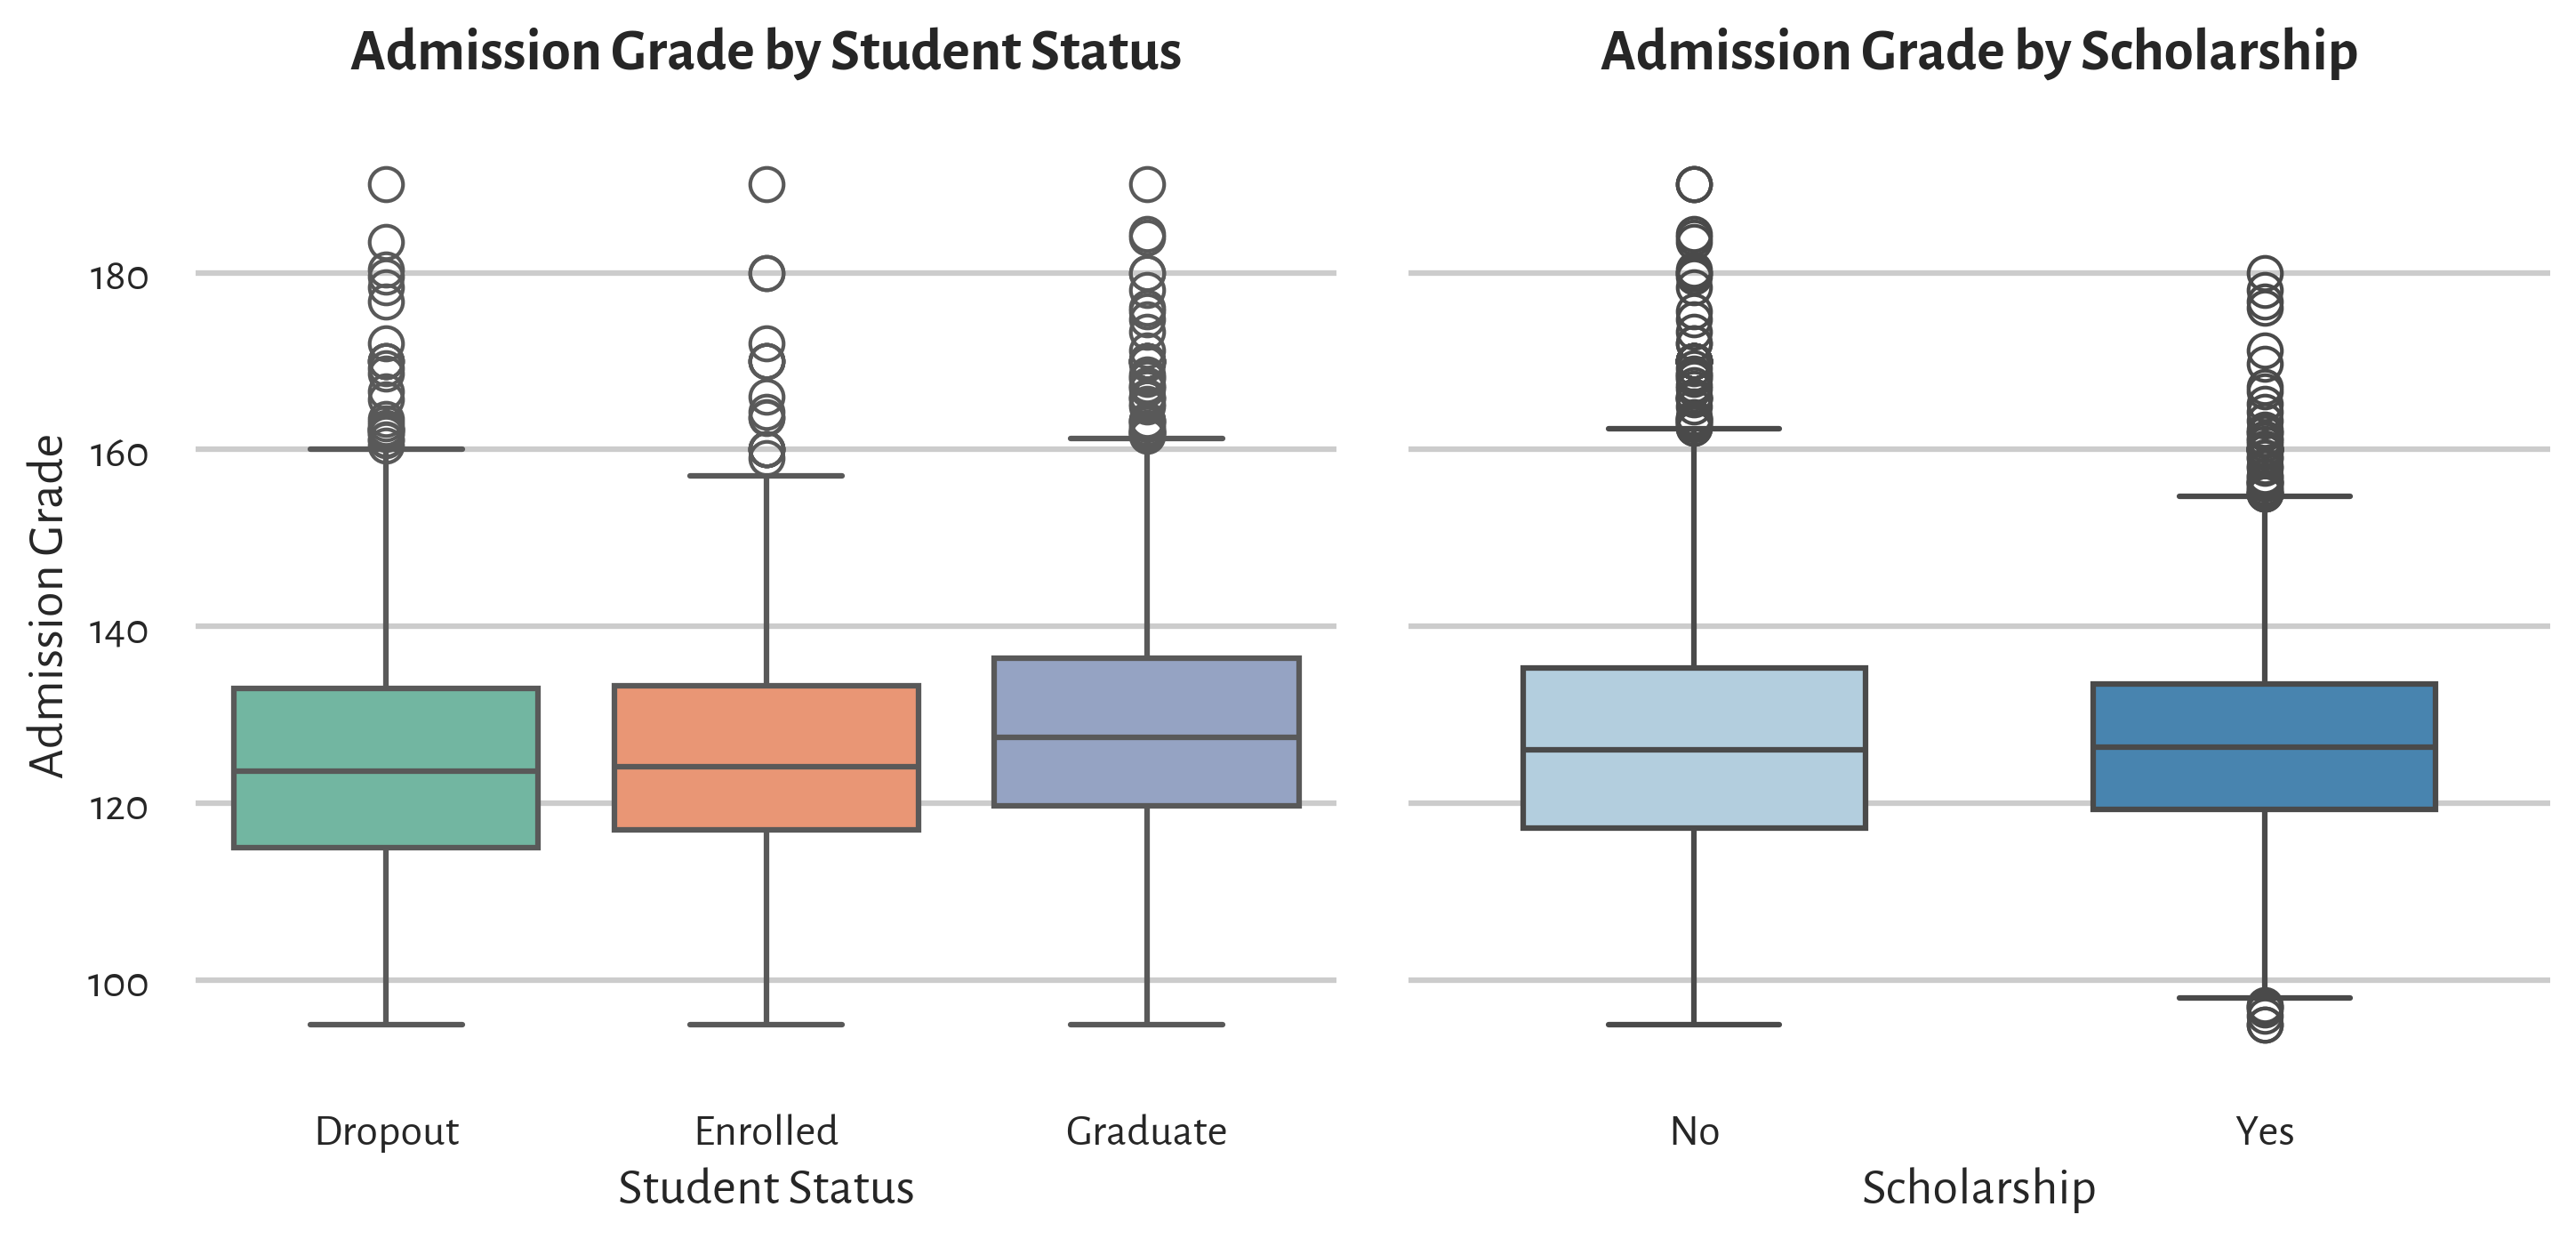
\includegraphics[width=1\textwidth]{Tex_Pictures/Graph_admission_grade.png} \\
     \end{center}
\end{frame}

\begin{frame}{Covariates: Family Background}
	\begin{center}
     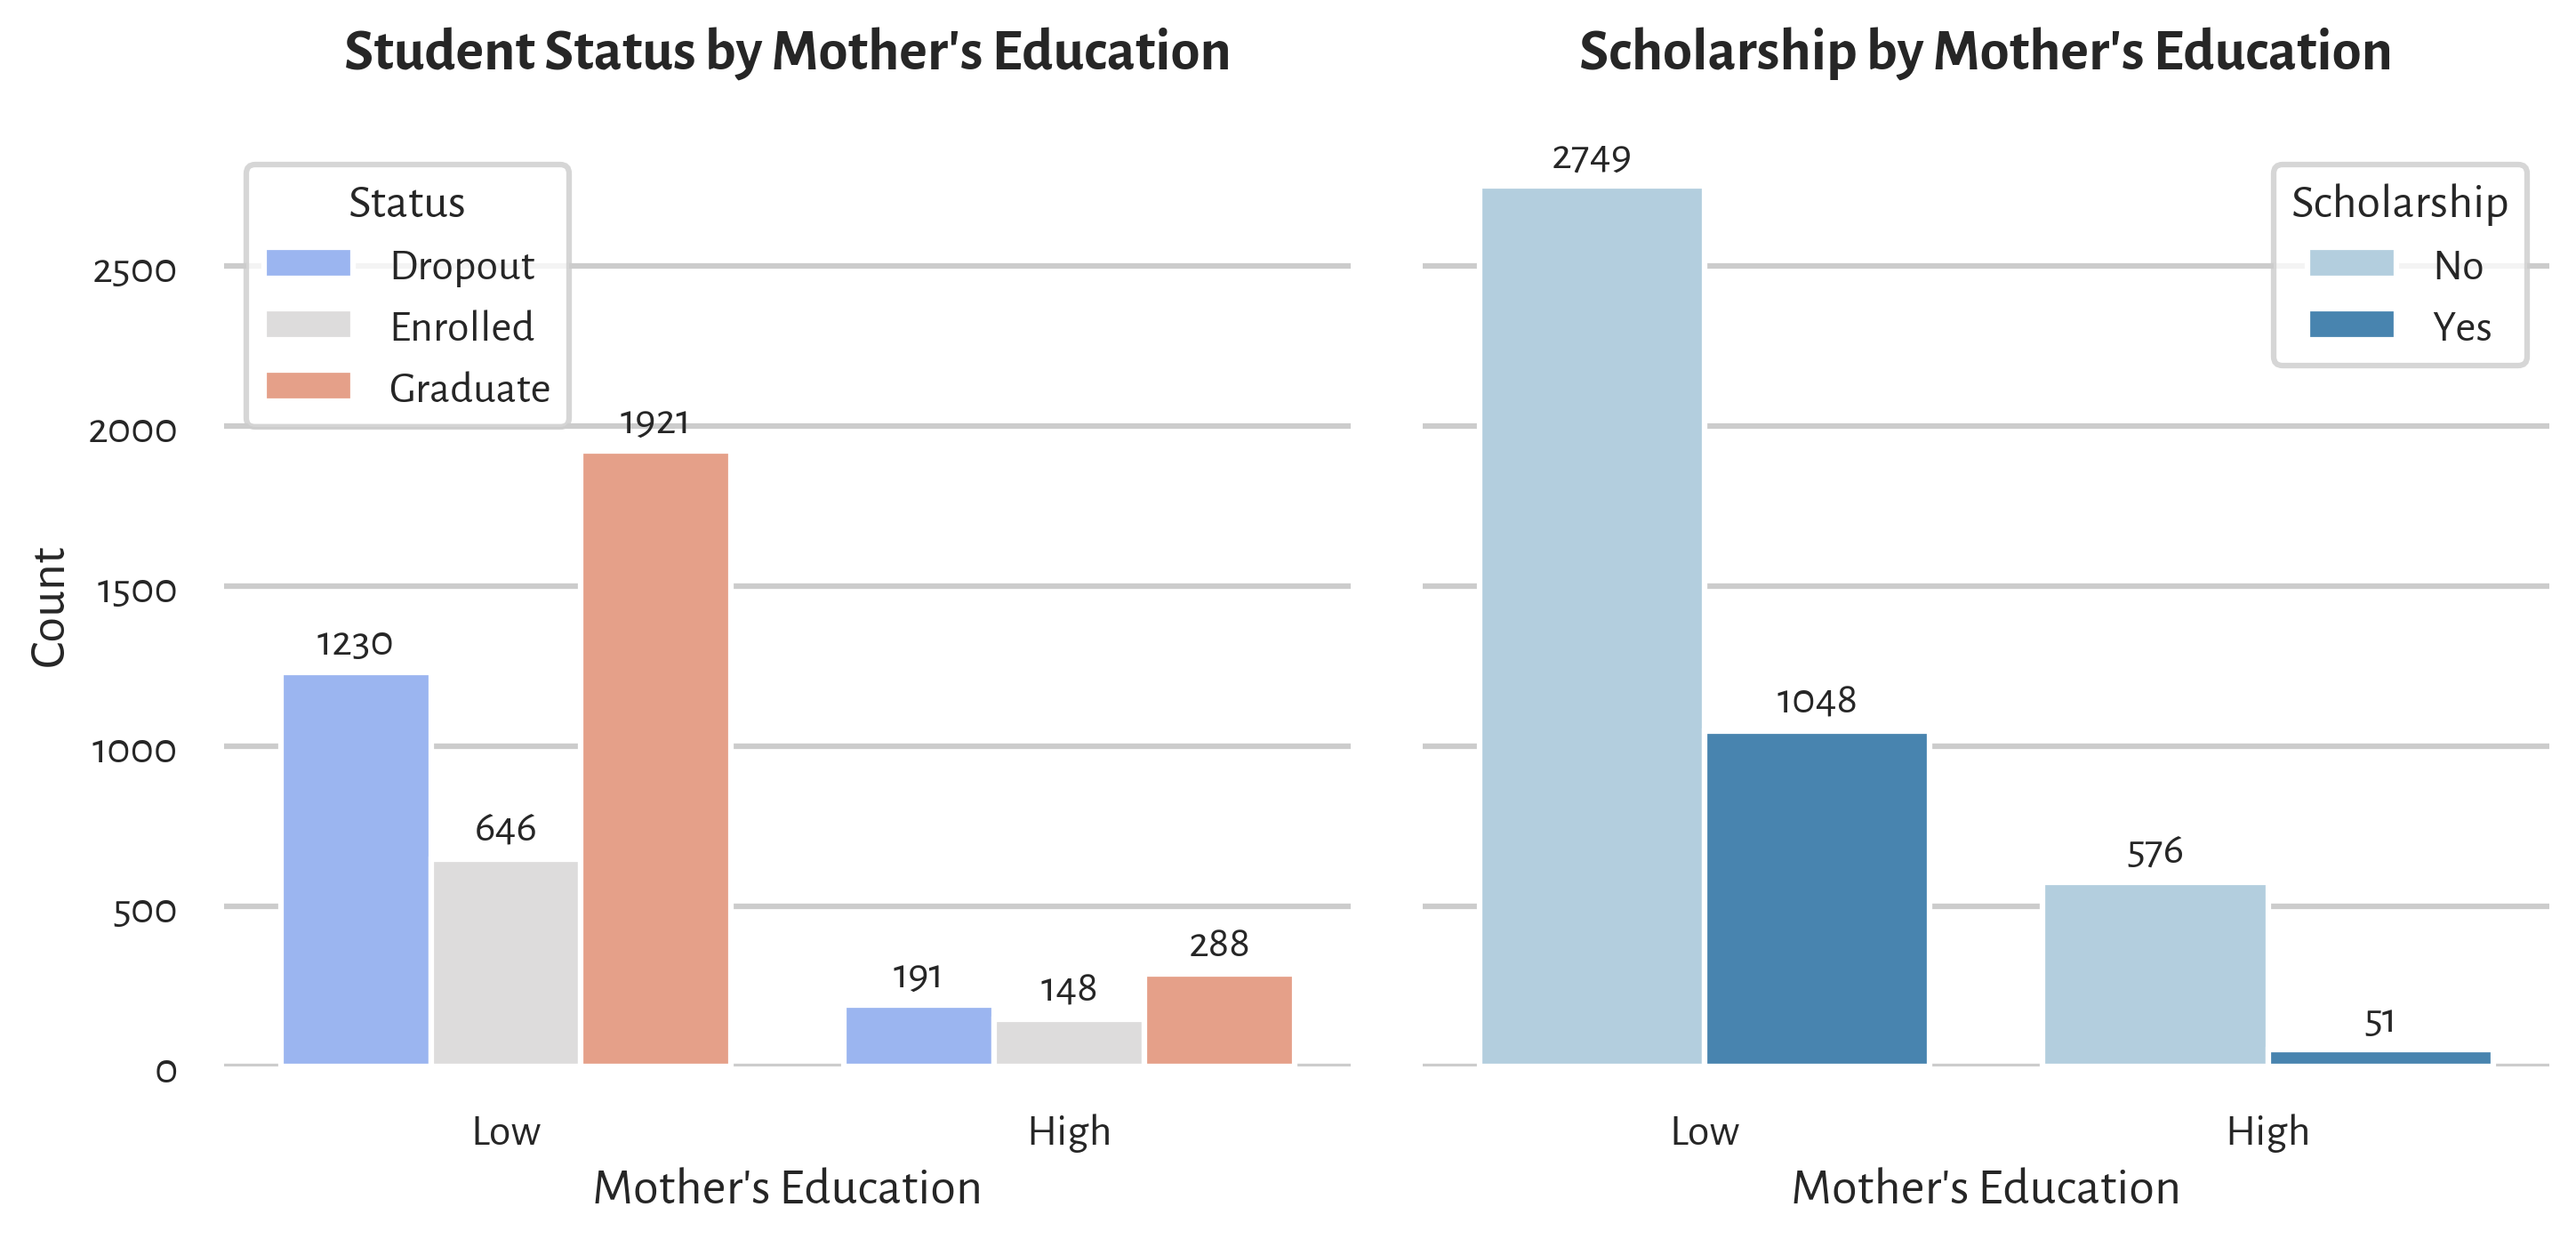
\includegraphics[width=1\textwidth]{Tex_Pictures/Graph_mother_educ}
     \end{center}
\end{frame}

\begin{frame}{Covariates: Gender}
	\begin{center}
     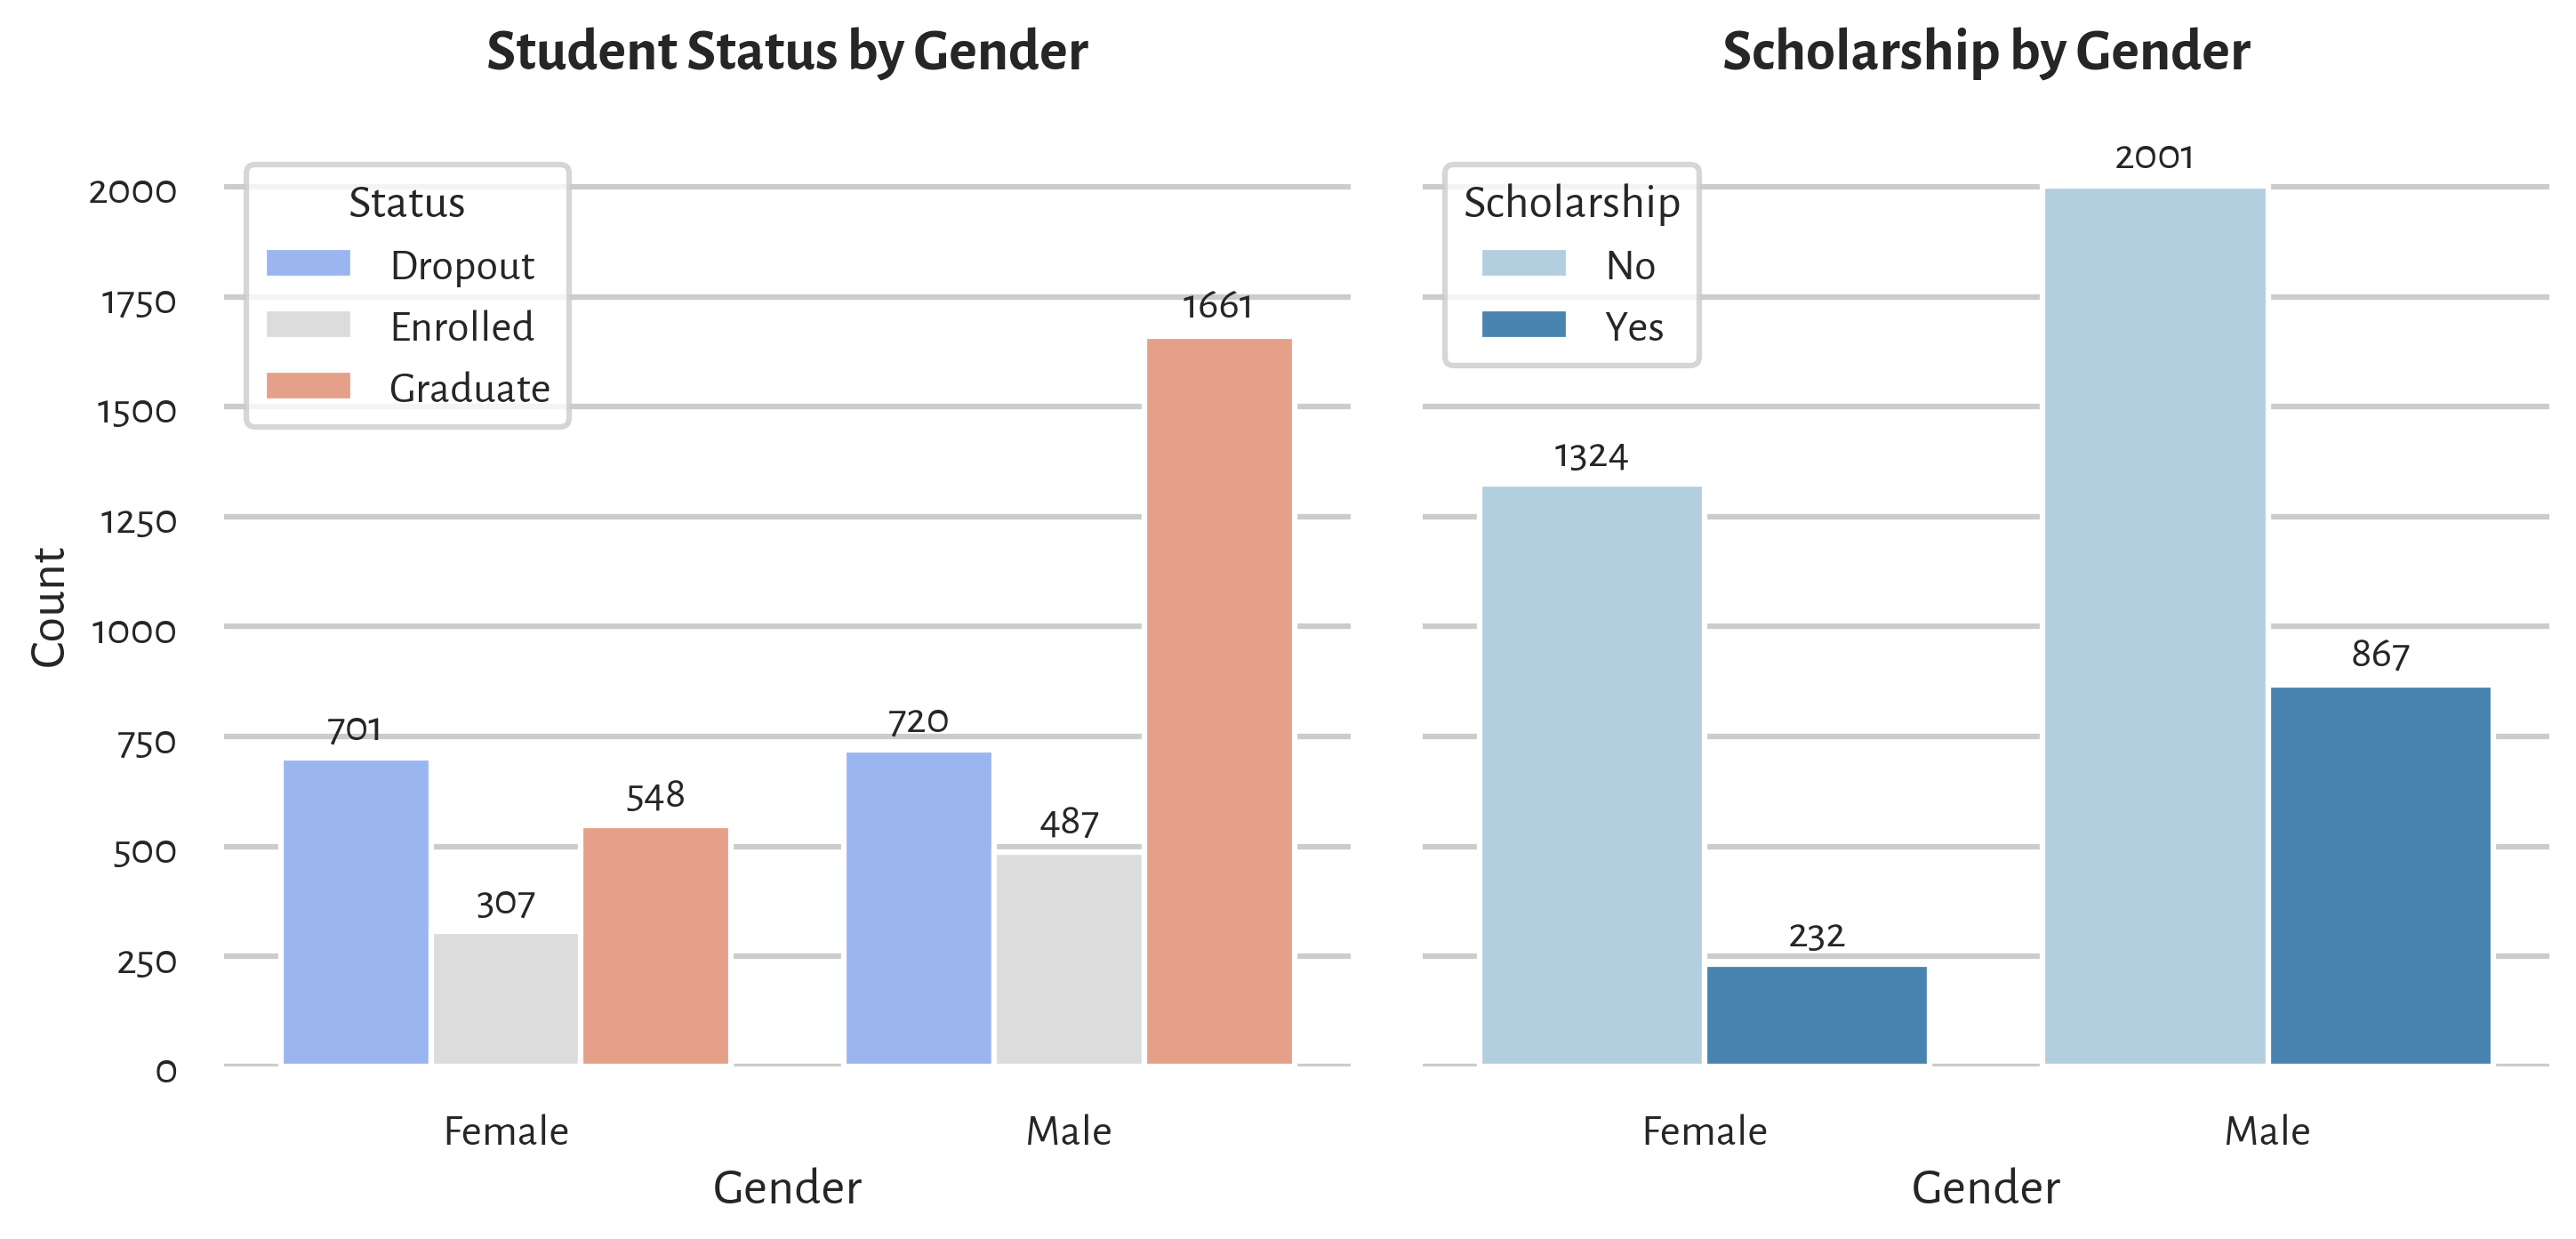
\includegraphics[width=1\textwidth]{Tex_Pictures/Graph_gender.png}
     \end{center}
\end{frame}

% ---------------------------------------
% Section Causal Graph and Covariate Selection
% ---------------------------------------

\section{4. Causal Graph and Covariate Selection}

\begin{frame}{Simplified Causal Graph}
	\begin{center}
     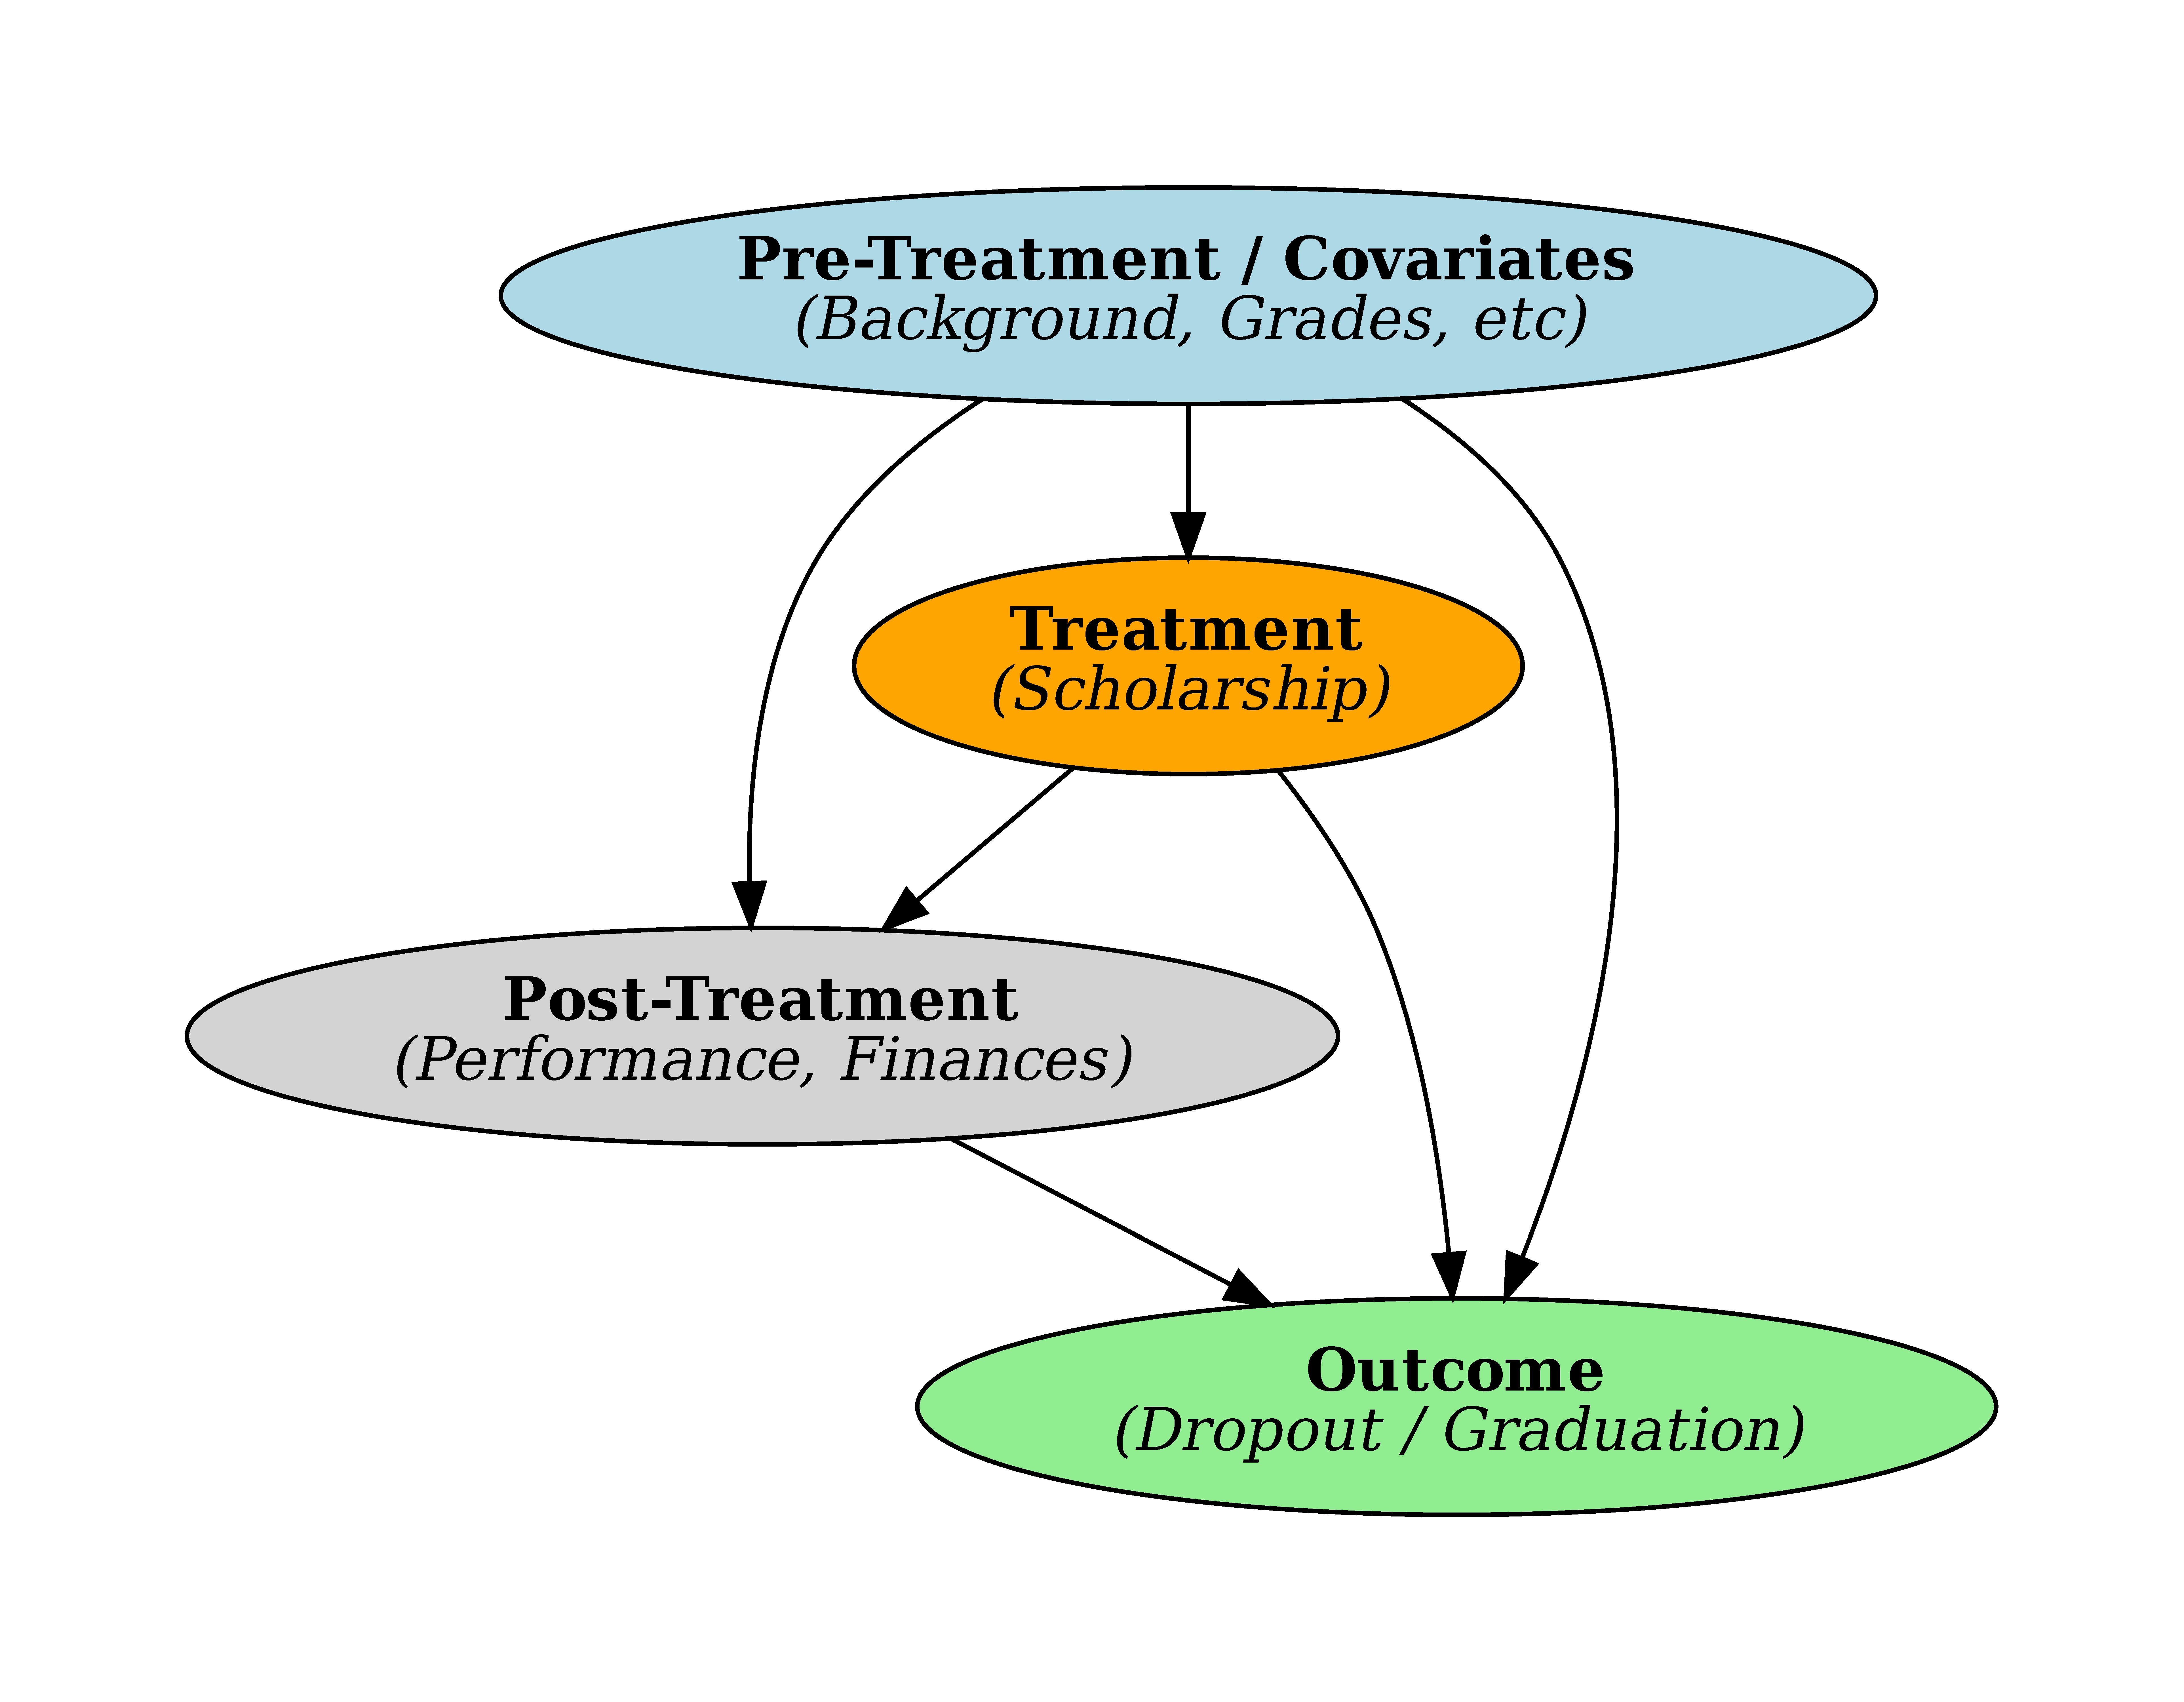
\includegraphics[width=0.6\textwidth]{Tex_Pictures/DAG_simple.png}
     \end{center}
\end{frame}

\begin{frame}{Simplified Causal Graph \& Relevant Paths}
	 \begin{columns}
	\begin{column}{0.58\textwidth}

\textbf{Three relevant paths between \\ Treatment (incoming) \& Outcome}
\small{
\begin{itemize}
    \item [1.] Treatment (incoming) $\leftarrow$ Covariates $\rightarrow$ Outcome
    \item [2.] Treatment (incoming) $\leftarrow$ Covariates $\rightarrow$ Post-Treatment $\rightarrow$ Outcome
    \item [3.] Treatment (incoming) $\leftarrow$ Covariates $\rightarrow$ Post-Treatment $\leftarrow$ Treatment (outgoing) $\rightarrow$ Outcome
\end{itemize}}
\begin{itemize}
	\item [$\Rightarrow$] All paths are blocked simultaneously by conditioning on the covariates, but NOT conditioning on the post-treatment effects.
\end{itemize}
  \end{column}

	\begin{column}{0.45\textwidth}
	\hspace*{-0.5cm}
    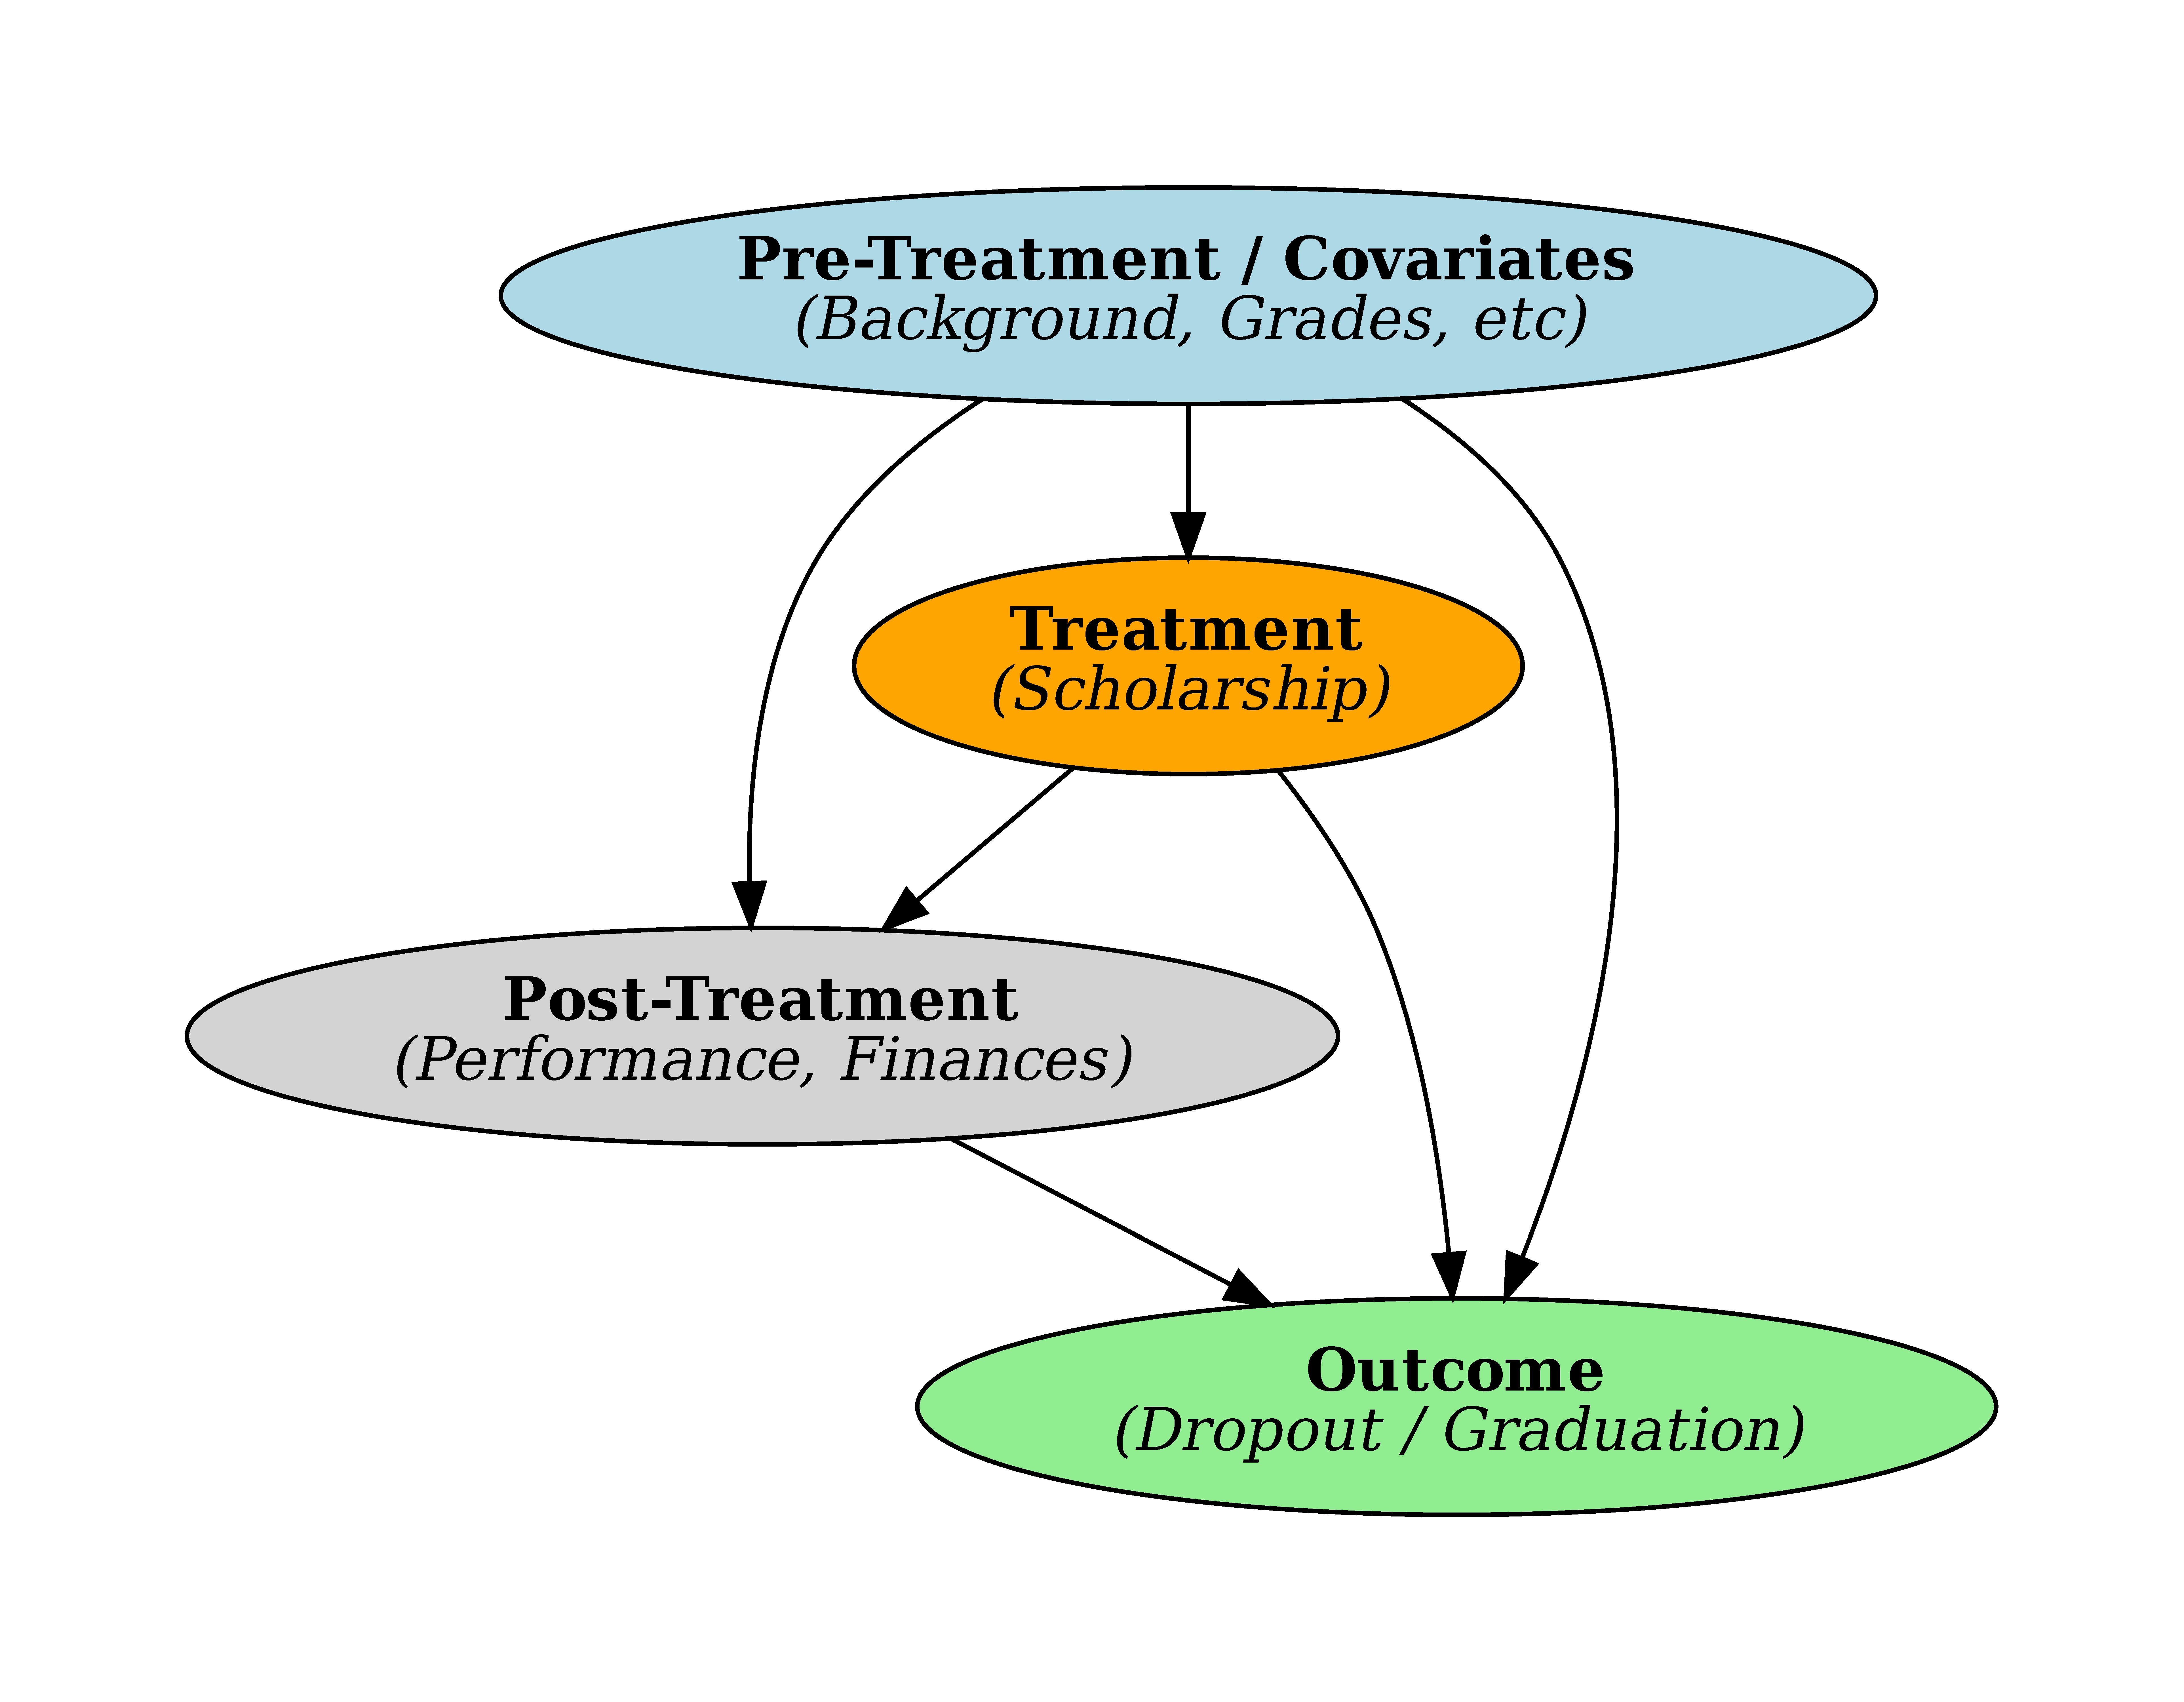
\includegraphics[width=1.1\textwidth]{Tex_Pictures/DAG_simple.png}

	\end{column}

\end{columns}
\end{frame}

\begin{frame}{Covariate selection}

	\textbf{37 features in the dataset, including one treatment and one target}
	\vspace{10pt}
	
	\begin{tabularx}{\textwidth}{X | X | X}
	\textbf{Pre-treatment (14)}  & \textbf{Post-treatment (14)} & \textbf{Unsuitable (7)} \\[0.5ex]
	\hline \hline 
	\parbox[t]{4cm}{\vspace{-12pt} \begin{itemize}
	[label=--,leftmargin=1.2em,itemsep=1pt,topsep=2pt]
    \item Academic performance before university
    \item Family background
    \item Economic context
    \item Individual characteristics (age, gender, etc.)
	\end{itemize}} 

	&
	\parbox[t]{4cm}{
	\vspace{-12pt}
	\begin{itemize}[label=--,leftmargin=1.2em,itemsep=1pt,topsep=2pt]
    	\item Academic performance during university
    	\item Financial situation during university
	\end{itemize}}
	&
	\parbox[t]{4cm}{\vspace{-12pt} 
	\begin{itemize}[label=--,leftmargin=1.2em,itemsep=1pt,topsep=2pt]
    	\item Marital status
    	\item Course selection
    	\item Parental occupation
    	\item Nationality
    	\item Etc.
	\end{itemize}} 
	\end{tabularx}


\end{frame}

\begin{frame}{Full Causal Graph}
	\begin{center}
	\textbf{Directed Acyclic Graph (DAG) of the Causal Relationships}
	\hspace*{-1cm}
     \includegraphics[width=1.15\textwidth]{Tex_Pictures/DAG_extended.png}
     \end{center}
\end{frame}

\begin{frame}{Assumptions}
\textbf{Main Assumptions for Identification of the Effect}
\begin{itemize}
    \item [1.] \textbf{Ignorability (Conditional Independence):} \\No unmeasured factors that both influence scholarship status and dropout rate.
    \item [2.] \textbf{Positivity:} \\There should be an overlap in characteristics – for any combination of covariates, there are both scholarship and non-scholarship students.
    \item [3.] \textbf{No interference:} \\One student’s scholarship does not directly affect another’s outcome.
\end{itemize}

\end{frame}


% ---------------------------------------
% Section Double Post Lasso
% ---------------------------------------
\section{5. Causal Effect Estimation Using Double Post Lasso}

\begin{frame}{Steps of the Double Post Lasso (DPL) Procedure}
\textbf{Double Post-Lasso Identifies the Causal Effect of Scholarships by Selecting Key Confounders}

\begin{itemize}
	\item[1.] Select controls for the outcome: Lasso regression of outcome $Y$ on covariates $X$ \\$\rightarrow$ \textit{selects predictors of student success}
	\item[2.] Select controls for the treatment: Lasso regression of treatment $D$ (scholarship) on $X$ \\ $\rightarrow$ s\textit{elects predictors of scholarship assignment}
	\item[3.] Union of selected covariates: Take the union of covariates from Steps 1 \& 2 \\ $\rightarrow$ \textit{ensures we control for all relevant confounders}
	\item[4.] Final OLS Regression Regress $Y$ on $D$ and the selected covariates
\end{itemize}

\begin{itemize}
	\item[$\Rightarrow$] DPL allows valid causal inference by \textit{selecting only the covariates that matter} for treatment and outcome, \textit{avoiding overfitting and omitted variable bias}.
\end{itemize}
\vspace{-10pt}
\end{frame}

\begin{frame}{Results Double Post Lasso: RQ1 (Dropout)}
\vspace{20pt}
    \begin{alertblock}{RQ1}
	Does receiving a scholarship \textbf{reduce} the likelihood of \textbf{dropping out} within 3 years?
	\end{alertblock}

\begin{block}{Results}
\begin{itemize}[label=--,itemsep=1pt,topsep=2pt]
	\item Covariates selected by Lasso: Outcome model - 4, Treatment model - 9
	\item Covariates in final union used for OLS: 10
	\item Estimated ATE of Scholarship on Dropout: -0.2030 (s.e. 0.0159) (p-value 0.0000***)
\end{itemize}
\end{block}

\begin{exampleblock}{Conclusion}
\vspace{-3pt}
\begin{itemize}
	\item [$\Rightarrow$]Receiving a scholarship \textit{significantly} \textbf{reduces} the probability of \textbf{dropout} within 3 years \\ by 20.3 \%-points. 
\end{itemize}
\vspace{-3pt}
\end{exampleblock}

\end{frame}

\begin{frame}{Results Double Post Lasso: RQ2 (On-Time Graduation)}
\vspace{20pt}
\begin{alertblock}{RQ2}
	Does receiving a scholarship \textbf{increase} the likelihood of \textbf{graduating} within 3 years?
\end{alertblock}

\begin{block}{Results}
\begin{itemize}[label=--,itemsep=1pt,topsep=2pt]
	\item Covariates selected by Lasso: Outcome model - 10, Treatment model - 9
	\item Covariates in final union used for OLS: 12
	\item Estimated ATE of Scholarship on Graduation: -0.2789 (s.e. 0.0169) (p-value 0.0000***)
\end{itemize}
\end{block}

\begin{exampleblock}{Conclusion}
\vspace{-3pt}
\begin{itemize}
	\item [$\Rightarrow$]Receiving a scholarship \textit{significantly} \textbf{increases} the probability of \textbf{graduating} within \\ 3 years by 27.8 \%-points.
\end{itemize}
\vspace{-3pt}	
\end{exampleblock}

\end{frame}

% ---------------------------------------
% Section Double Machine Learning
% ---------------------------------------
\section{6. Causal Effect Estimation Using Double Machine Learning}

\begin{frame}{Steps of the Double Machine Learning (DML) Procedure}
\textbf{Double Machine Learning Estimates the Causal Effect Using Flexible ML Models}
\vspace{-3pt}
\begin{itemize}
    \item[1.] Normalize numerical covariates \\ 
    $\rightarrow$ \textit{ensures comparability and prepares data for ML models}
    \item[2.] Estimate the propensity score: Random Forest classifier models treatment $D$ on $X$ \\ 
    $\rightarrow$ \textit{learns who receives scholarships: } $P(D = 1 \mid X)$  
    \item[3.] Estimate the outcome model: Lasso regression with cross-validation predicts $Y$ from $X$ \\ 
    $\rightarrow$ \textit{models expected student outcome: } $E[Y \mid X]$
    \item[4.] Apply DoubleMLPLR (Partially Linear Regression) to estimate the ATE \\ 
    $\rightarrow$ \textit{controls for confounding via orthogonalization and cross-fitting}
\end{itemize}
\vspace{-3pt}
\begin{itemize}
    \item[$\Rightarrow$] DML enables robust causal inference by using \textit{machine learning to flexibly control for high-dimensional confounders}, while correcting for overfitting.
\end{itemize}
\vspace{-10pt}
\end{frame}



\begin{frame}{Results Double Machine Learning: RQ1 (Dropout)}
\vspace{20pt}
    \begin{alertblock}{RQ1}
	Does receiving a scholarship \textbf{reduce} the likelihood of \textbf{dropping out} within 3 years?
	\end{alertblock}

\begin{block}{Results}
\begin{itemize}[label=--,itemsep=1pt,topsep=2pt]
	\item Estimated Treatment Effect: -0.1701 (17\% decrease) (s.e. 0.0137)
	\item 95\% Confidence Interval: [-0.1969, -0.1432]
	\item P-value: 0.0000 (***) (t-stat: -12.4159)
\end{itemize}
\end{block}

\begin{exampleblock}{Conclusion}
\vspace{-3pt}
\begin{itemize}
	\item [$\Rightarrow$]Receiving a scholarship \textit{significantly} \textbf{reduces} the probability of \textbf{dropout} within 3 years \\ by 17.6 \%-points. 
\end{itemize}
\vspace{-3pt}
\end{exampleblock}

\end{frame}

\begin{frame}{Results Double Machine Learning: RQ2 (On-Time Graduation)}
\vspace{20pt}
\begin{alertblock}{RQ2}
	Does receiving a scholarship \textbf{increase} the likelihood of \textbf{graduating} within 3 years?
\end{alertblock}

\begin{block}{Results}
\begin{itemize}[label=--,itemsep=1pt,topsep=2pt]
	\item Estimated Treatment Effect: 0.2348 (23\% increase) (s.e. 0.0162)
	\item 95\% Confidence Interval: [0.2031, 0.2666]
	\item P-value: 0.0000 (***) (t-stat: 14.4859)
\end{itemize}
\end{block}

\begin{exampleblock}{Conclusion}
\vspace{-3pt}
\begin{itemize}
	\item [$\Rightarrow$]Receiving a scholarship \textit{significantly} \textbf{increases} the probability of \textbf{graduating} within \\ 3 years by 23.5 \%-points.
\end{itemize}
\vspace{-3pt}
	
\end{exampleblock}

\end{frame}



% ---------------------------------------
% MARIMAR SECTION
% ---------------------------------------

\section{7. Parameter/model selection for the statistical estimator}

\begin{frame}{STEPS}

\begin{itemize}
    \item[1.] Data preprocessing

    \item[2.] 3 Learners for outcomes (Linear, Lasso, Randomforest) and 3 others learners for treatment (Logistic, Lasso, random forest classifier)
    \item[3.] Combines learners to improve predictions with stacking regressor: \[         \hat{Y_i} = \sum_{j=1}^{3} w_j \hat{Y}_{ij}      \text{  }  \text{ and } \text{  }  \hat{D_i} = \sum_{j=1}^{3} v_j \hat{D}_{ij}         \] 
    where \( w_j \)  and \( v_j \) are learned through LassoCV.
        \item A robust approach to estimate \( E[Y|X] \) and \( E[D|X] \).
    \item[4.] DML estimates 
    \item But for DPL just cross validation with 10 repetitions
\end{itemize}
    
\end{frame}


\begin{frame}{RESULTS with cross validation}

\vspace{20pt}
\begin{alertblock}{DML}
	\begin{itemize}[label=--,itemsep=1pt,topsep=2pt]
	\item Estimated Treatment Effect on dropout: -0.201 VS -0.17,\\ with a wider confidence interval [-0.228, -0.173] VS   [-0.197, -0.143]
	\item Estimated Treatment Effect on graduate within 3 years:  0.273 VS 0.235,\\ 
    with a wider confidence interval [0.240, 0.306] VS [0.203, 0.267].
	
\end{itemize}
\end{alertblock}


\begin{exampleblock}{Conclusion}
\vspace{-2pt}
The effect appears stronger in absolute value, which suggests better handling of data variability through stacking and cross-fitting
\begin{itemize}

    \item [$\Rightarrow$]Receiving a scholarship \textit{significantly} \textbf{decreases} the probability of \textbf{dropout} by 20.1 \%-points.
    \item [$\Rightarrow$]Receiving a scholarship \textit{significantly} \textbf{increases} the probability of \textbf{graduating} within \\ 3 years by 27.5 \%-points.
\end{itemize}
\vspace{-3pt}
	
\end{exampleblock}

    
\end{frame}



\begin{frame}{RESULTS with cross validation}

\vspace{20pt}
\begin{alertblock}{DPL}
	\begin{itemize}[label=--,itemsep=1pt,topsep=2pt]
	\item Estimated Treatment Effect on dropout: -0.220 VS ,\\ with a wider confidence interval [-0.246, -0.194] VS   
	\item Estimated Treatment Effect on graduate within 3 years:  0.313 VS ,\\ 
    with a wider confidence interval [0.282, 0.344] VS .

\end{itemize}
\end{alertblock}


\begin{exampleblock}{Conclusion}
\vspace{-2pt}
DML with Cross-Fitting  leads to stronger effects and more reliable inference. This method better controls for confounders and prevents overfitting, making it the \textbf{preferred approach for causal estimation} in this context.

\vspace{-3pt}
	
\end{exampleblock}

    
\end{frame}


\section{8. Heterogeneous Treatment Effects}

\begin{frame}{STEPS}

\textbf{RQ: Does the impact of scholarships differ for some subgroups of students? \\}
subgroups defined by: gender, age at enrollment, previous qualification grade , admission grade, mother education and father education

\begin{itemize}
    \item[1.] \textbf{Step 1}: Estimate the potential outcomes for the treatment and control groups using two separate learners (XGboost here).

gC(Z): Predicted outcome when treated as control (D=0).

gT(Z): Predicted outcome when treated as treatment (D=1).


    \item[2.] \textbf{Step 2}: Calculate the treatment effect for each observation as the difference between the predicted outcomes:

Treatment Effect= gT(Z)- gC(Z) for each indicual. This is the raw treatment effect.


    \item[3.] \textbf{Step 3} : Regress the treatment effect on the covariates X (Lasso) : CATE(X)
\end{itemize}

    
\end{frame}
    




\begin{frame}{Intermediate results}

\begin{figure}[h!]
    %\centering
    \begin{minipage}[b]{0.45\textwidth}
        
        \caption{Distribution of estimatesd HE on droupout}
        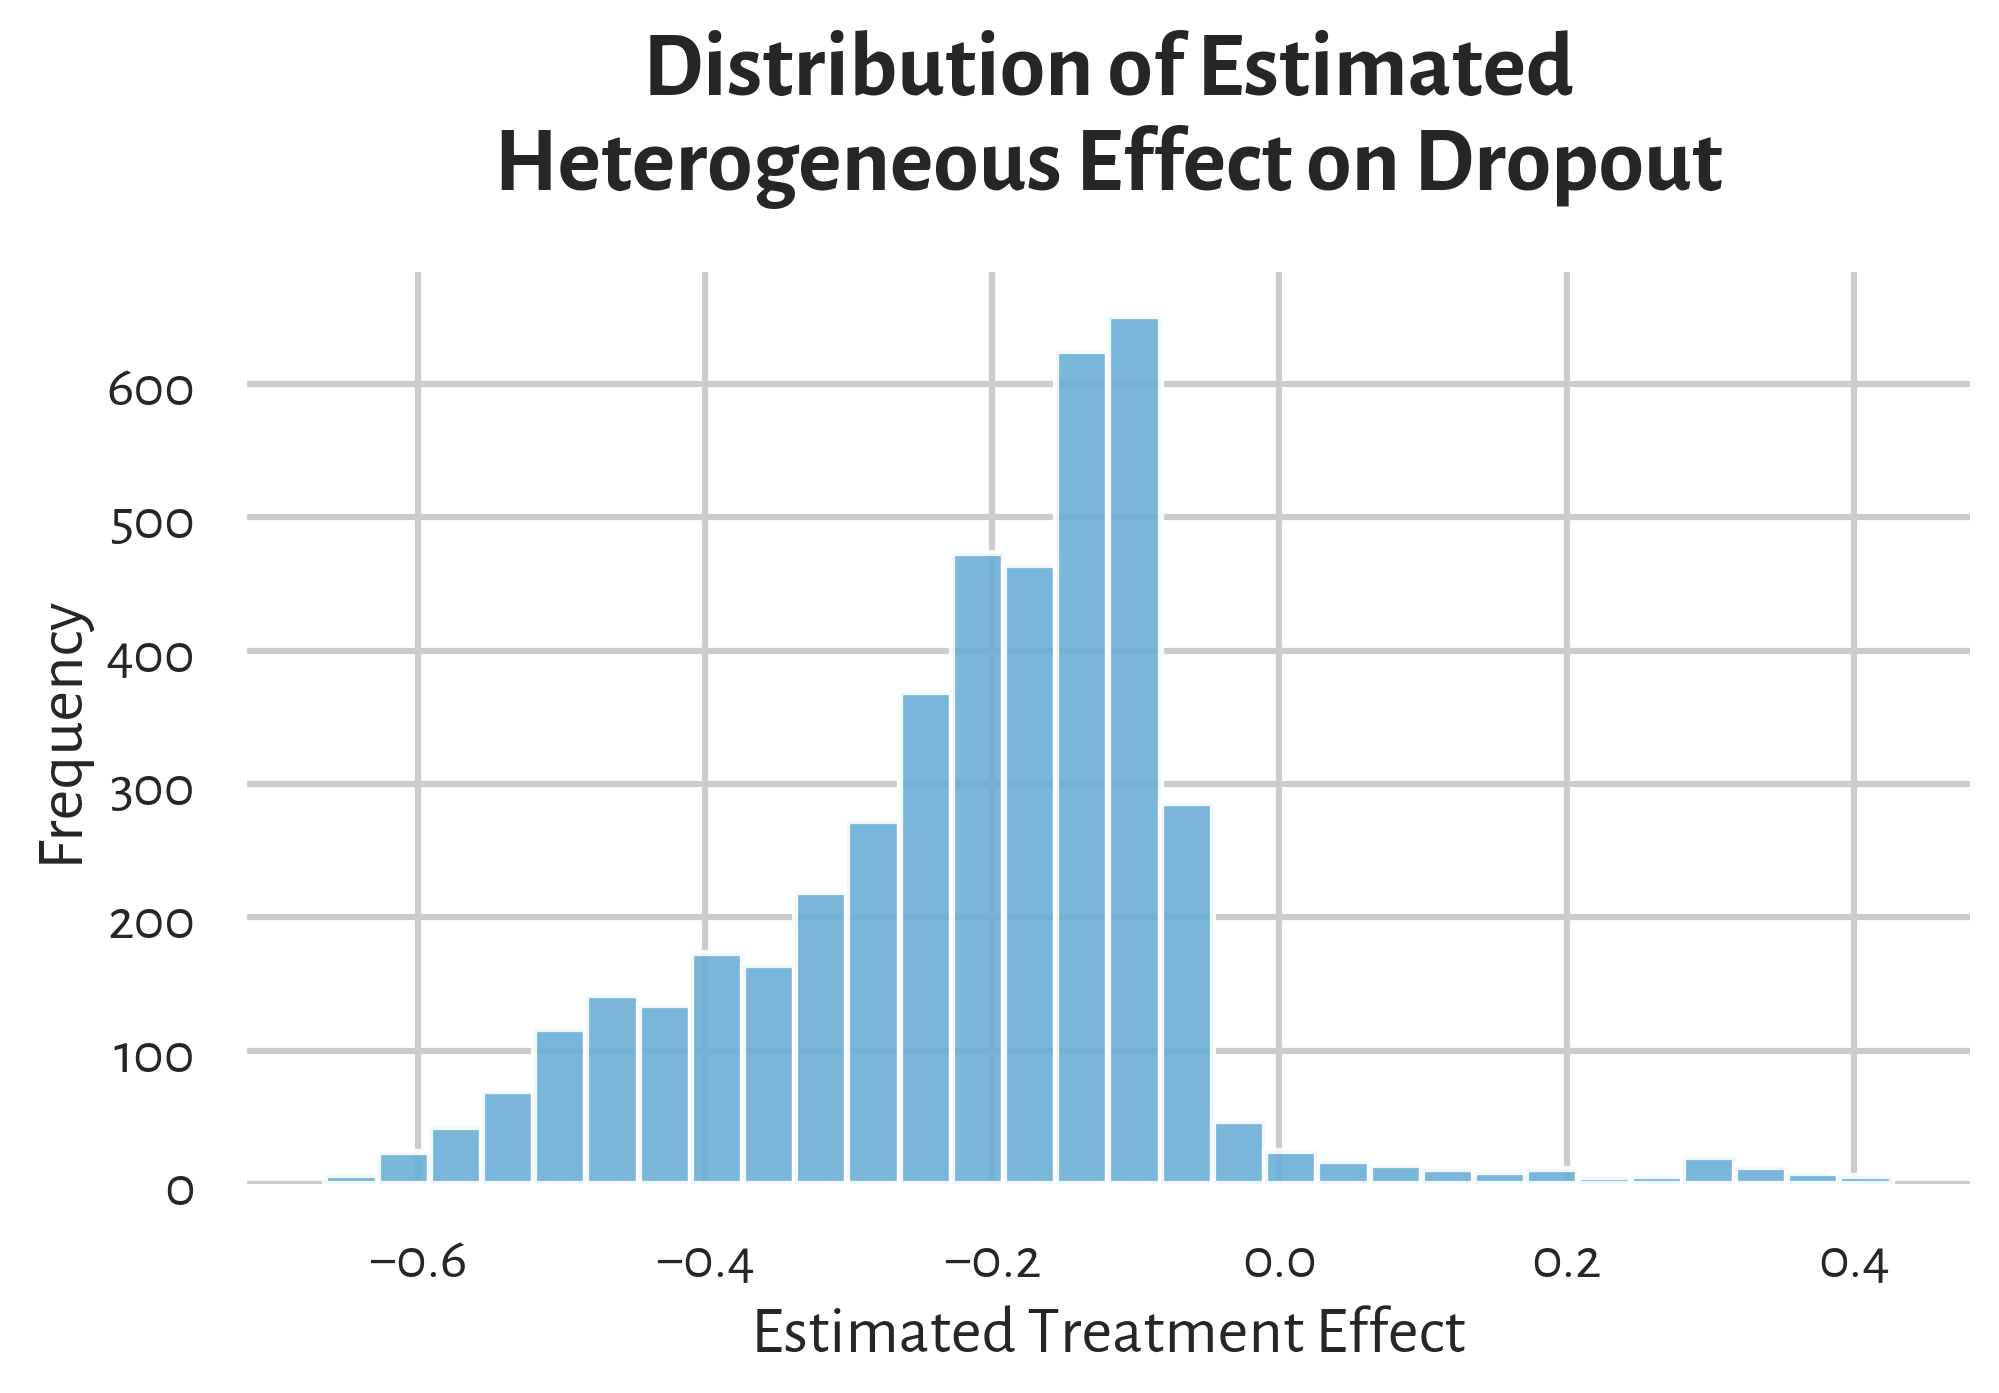
\includegraphics[width=1\linewidth]{Tex_Pictures/Distribution_of_TE_drop_out.png}

       \textbf{ CATE(X) = -0.215}
       
    \end{minipage}
    \hspace{0.05\textwidth}
    \begin{minipage}[b]{0.45\textwidth}
        %\centering
        \caption{Distribution of estimatesd HE on graduating}
        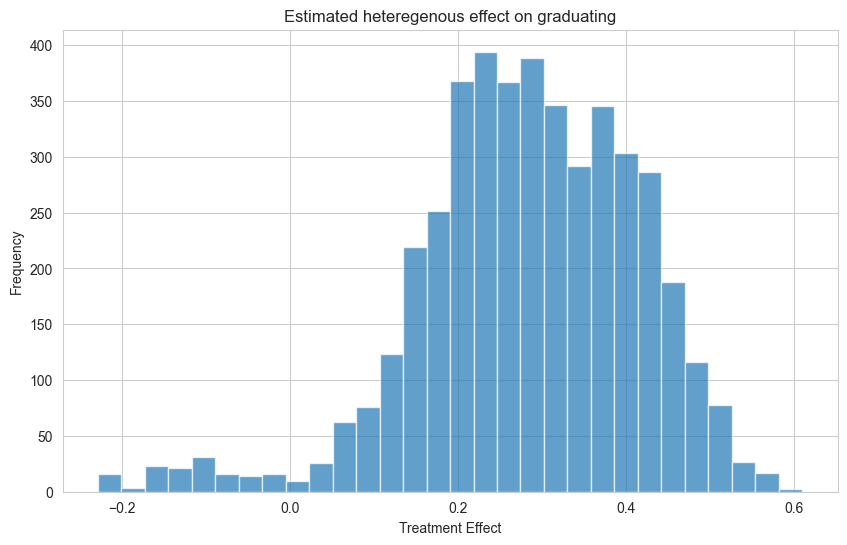
\includegraphics[width=1\linewidth]{Tex_Pictures/Distribution_TE_graduate.png}

         \textbf{ CATE(X) = 0.283}
       
    \end{minipage}
    
 \end{figure}   
\end{frame}




\begin{frame}{ Test of HE}

Consider the regression (with \( P(Z) \) known as \( P(D = 1 | Z) \)) and and B(z) is a proxy of E(Y(0)|Z):
\[
y = \alpha_0 + \alpha_1 B(Z) + \alpha_2 S(Z) + \beta_1 (D - P(Z)) + \beta_2 (D - P(Z))(S(Z) - S) + u
\]
\[ B_Z = \hat{gC(Z)}  \text{ and }  P_Z  \text{  }   \text{ estimated with XGboost classififer }\]


\begin{figure}[h!]
    %\centering
    \begin{minipage}[b]{0.45\textwidth}
        
       \begin{table}[h]
    \centering
    \begin{tabular}{l c c}
        \hline
        & \textbf{\(\hat\beta_2\) } & \textbf{CI} \\
        \hline
        Linear reg & -1.649 & [ -2.050, -1.245] \\
        Elasticnet & -1.36 & [-1.962, -1.251] \\
        \hline
    \end{tabular}
    \caption{Estimated \(\hat\beta_2\) coefficients on Dropout.}
    \label{tab:beta2_estimates}
\end{table}
    \end{minipage}
    \hspace{0.05\textwidth}
    \begin{minipage}[b]{0.45\textwidth}
        \begin{table}[h]
    \centering
    \begin{tabular}{l c c}
        \hline
        & \textbf{ (\(\hat\beta_2\))} & \textbf{CI} \\
        \hline
        Linear reg & -1.649 & [ -2.050, -1.245] \\
        Elasticnet & -1.36 & [-1.962, -1.251] \\
        \hline
    \end{tabular}
    \caption{Estimated \(\beta_2\) coefficients on graduating within 3 years}
    \label{tab:beta2_estimates}
\end{table}
       
    \end{minipage}
    
 \end{figure}   
\end{frame}





\begin{frame}{Results}

\begin{figure}[h!]  
        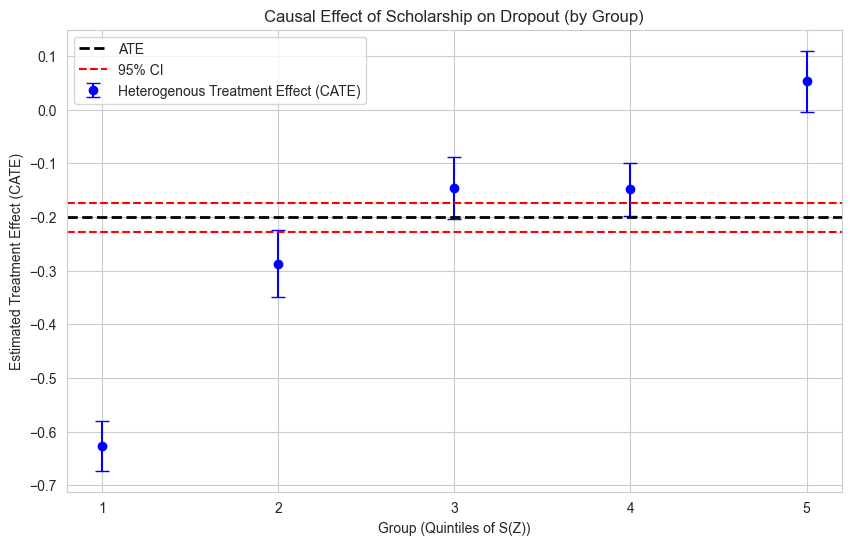
\includegraphics[width=0.8\linewidth]{Tex_Pictures/HE_quintile_dropout.png}

 \end{figure}   
\end{frame}



\begin{frame}{Results}
\begin{table}[h]
    \centering
    \begin{tabular}{l c c}
        \hline
        \textbf{Variable} & \textbf{First Quintile (Low S(Z))} & \textbf{Last Quintile (High S(Z))} \\
        \hline
        Gender & 54.124 & 12.090 \\
        Age at Enrollment & 30.966 & 20.149 \\
        Previous Qualification (Grade) & 129.587 & 139.921 \\
        Admission Grade & 123.785 & 134.141 \\
        Mother’s Education & 9.266 & 22.486 \\
        Father’s Education & 9.492 & 13.785 \\
        \hline
    \end{tabular}
    \caption{Comparison of Characteristics Between First and Last Quintiles of S(Z)}
    \label{tab:quintile_comparison}
\end{table}




 \textbf{Targeting students from disadvantaged backgrounds (older, lower parental education, and lower academic performance) could maximize its impact.}
\end{frame}


\begin{frame}{Results}

\begin{figure}[h!]  
        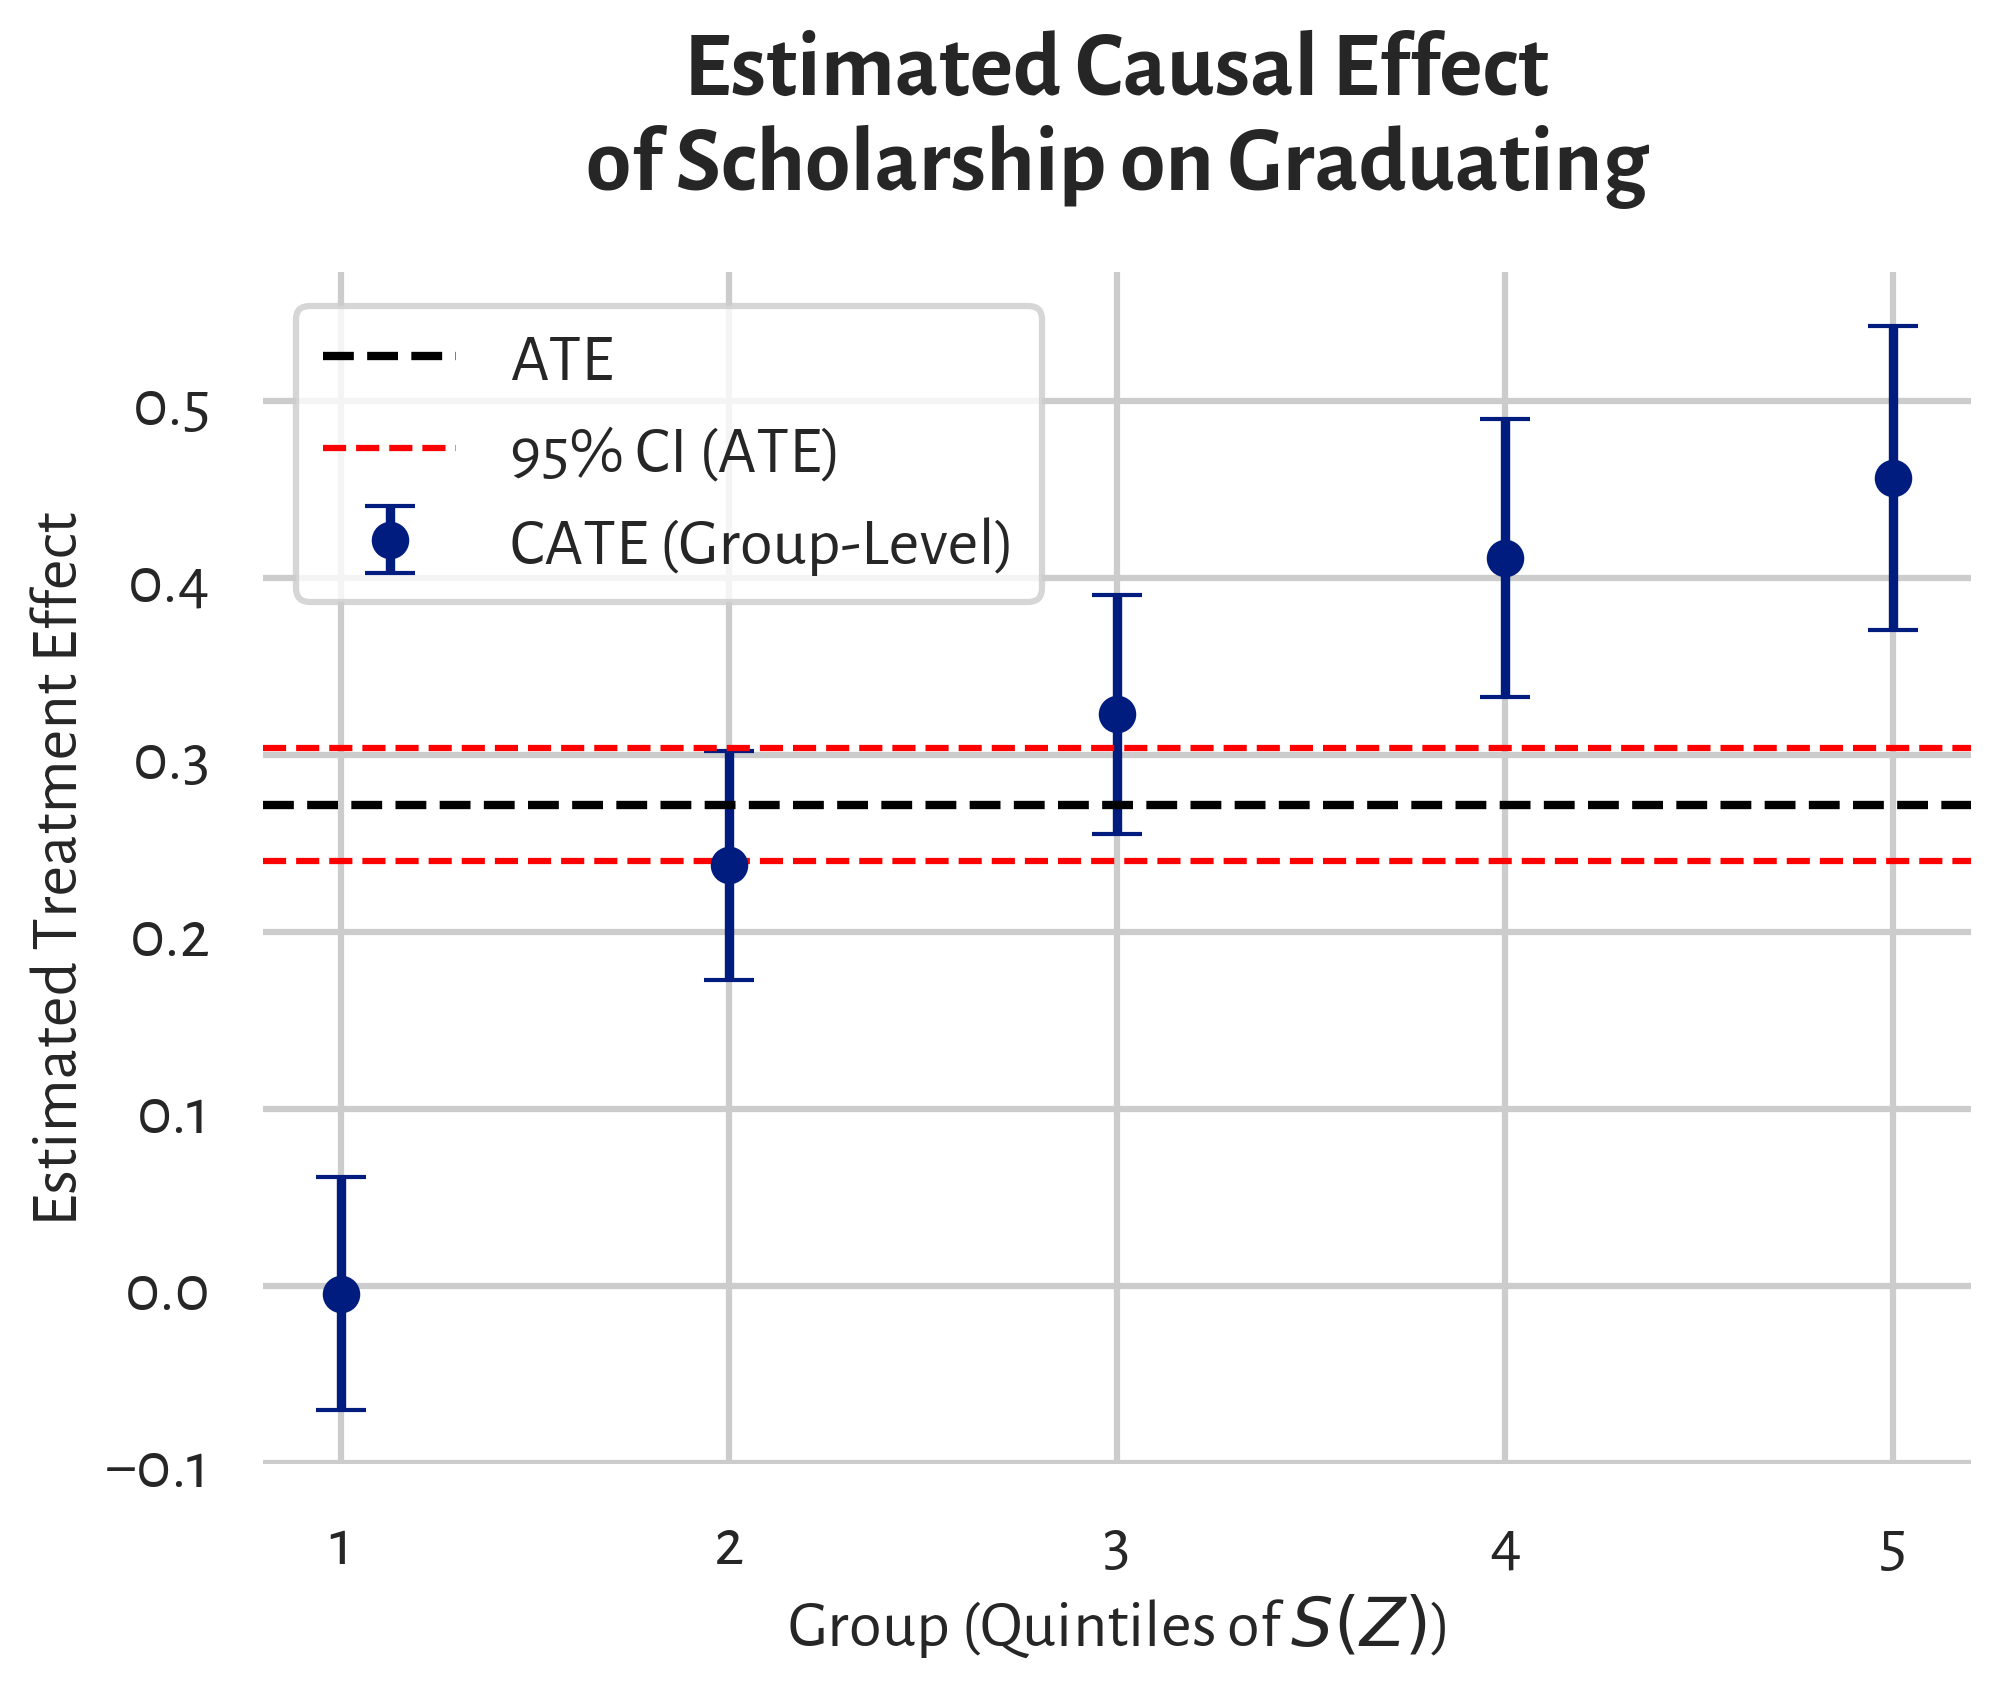
\includegraphics[width=0.8\linewidth]{Tex_Pictures/HE_quintile_graduating.png} 

 
 \end{figure}   
\end{frame}



\begin{frame}{Results}
\begin{table}[h]
    \centering
    \begin{tabular}{l c c}
        \hline
        \textbf{Variable} & \textbf{First Quintile (Low S(Z))} & \textbf{Last Quintile (High S(Z))} \\
        \hline
        Gender & 16.140 & 49.379 \\
        Age at Enrollment & 20.910 & 28.000 \\
        Previous Qualification (Grade) & 138.814 & 130.789 \\
        Admission Grade & 133.443 & 119.509 \\
        Mother’s Education & 10.835 & 12.316 \\
        Father’s Education & 7.449 & 11.299 \\
        \hline
    \end{tabular}
    \caption{Comparison of Characteristics Between First and Last Quintiles of S(Z)}
    \label{tab:quintile_comparison_2}
\end{table}



\textbf{Additional support beyond financial aid, such as mentoring or tutoring, may be needed for younger and more disadvantaged students}
\end{frame}


\begin{frame}{Gender-based Heterogeneity Analysis}
\vspace{5pt}
\begin{alertblock}{Approach}
	\textbf{Do scholarships affect male and female students differently?}
	\vspace{-10pt}
	\begin{itemize}[label=--,itemsep=1pt]
    \item Treatment effects estimated separately for male and female subgroups using DoubleML.
    \item Slightly stronger effects for female students across both outcomes.
\end{itemize}
\end{alertblock}
\vspace{5pt}
\begin{block}{Results}
\vspace{8pt}
\begin{columns}
\begin{column}{0.45\textwidth}
\textbf{RQ1 – Dropout (↓):}
\vspace{-3pt}
\begin{itemize}[label=--,itemsep=1pt]
    \item Males: \textbf{-0.1853 ± 0.0147}
    \item Females: \textbf{-0.2387 ± 0.0298}
\end{itemize}
\end{column}

\begin{column}{0.45\textwidth}
\textbf{RQ2 – Graduation (↑):}
\vspace{-3pt}
\begin{itemize}[label=--,itemsep=1pt]
    \item Males: \textbf{0.2630 ± 0.0180}
    \item Females: \textbf{0.2748 ± 0.0350}
\end{itemize}
\end{column}
\end{columns}
\vspace{4pt}
\end{block}



\vspace{5pt}
\begin{exampleblock}{Interpretation}
Scholarships \textbf{reduce dropout} and \textbf{improve graduation} outcomes for both genders, with a \textbf{slightly higher impact observed for female} students.

\end{exampleblock}

\end{frame}


% ---------------------------------------
% Section Robustness and Sensitivity Analysis
% ---------------------------------------
\section{9. Robustness and Sensitivity Analysis}


\begin{frame}{Check 1: Identifying Key Predictors of Student Outcomes using Feature Importance}
\centering
\textbf{Random Forest Feature Importance (Dropout and Scholarship Eligibility)}

\vspace{5pt}

\begin{columns}
\begin{column}{0.5\textwidth}
\centering
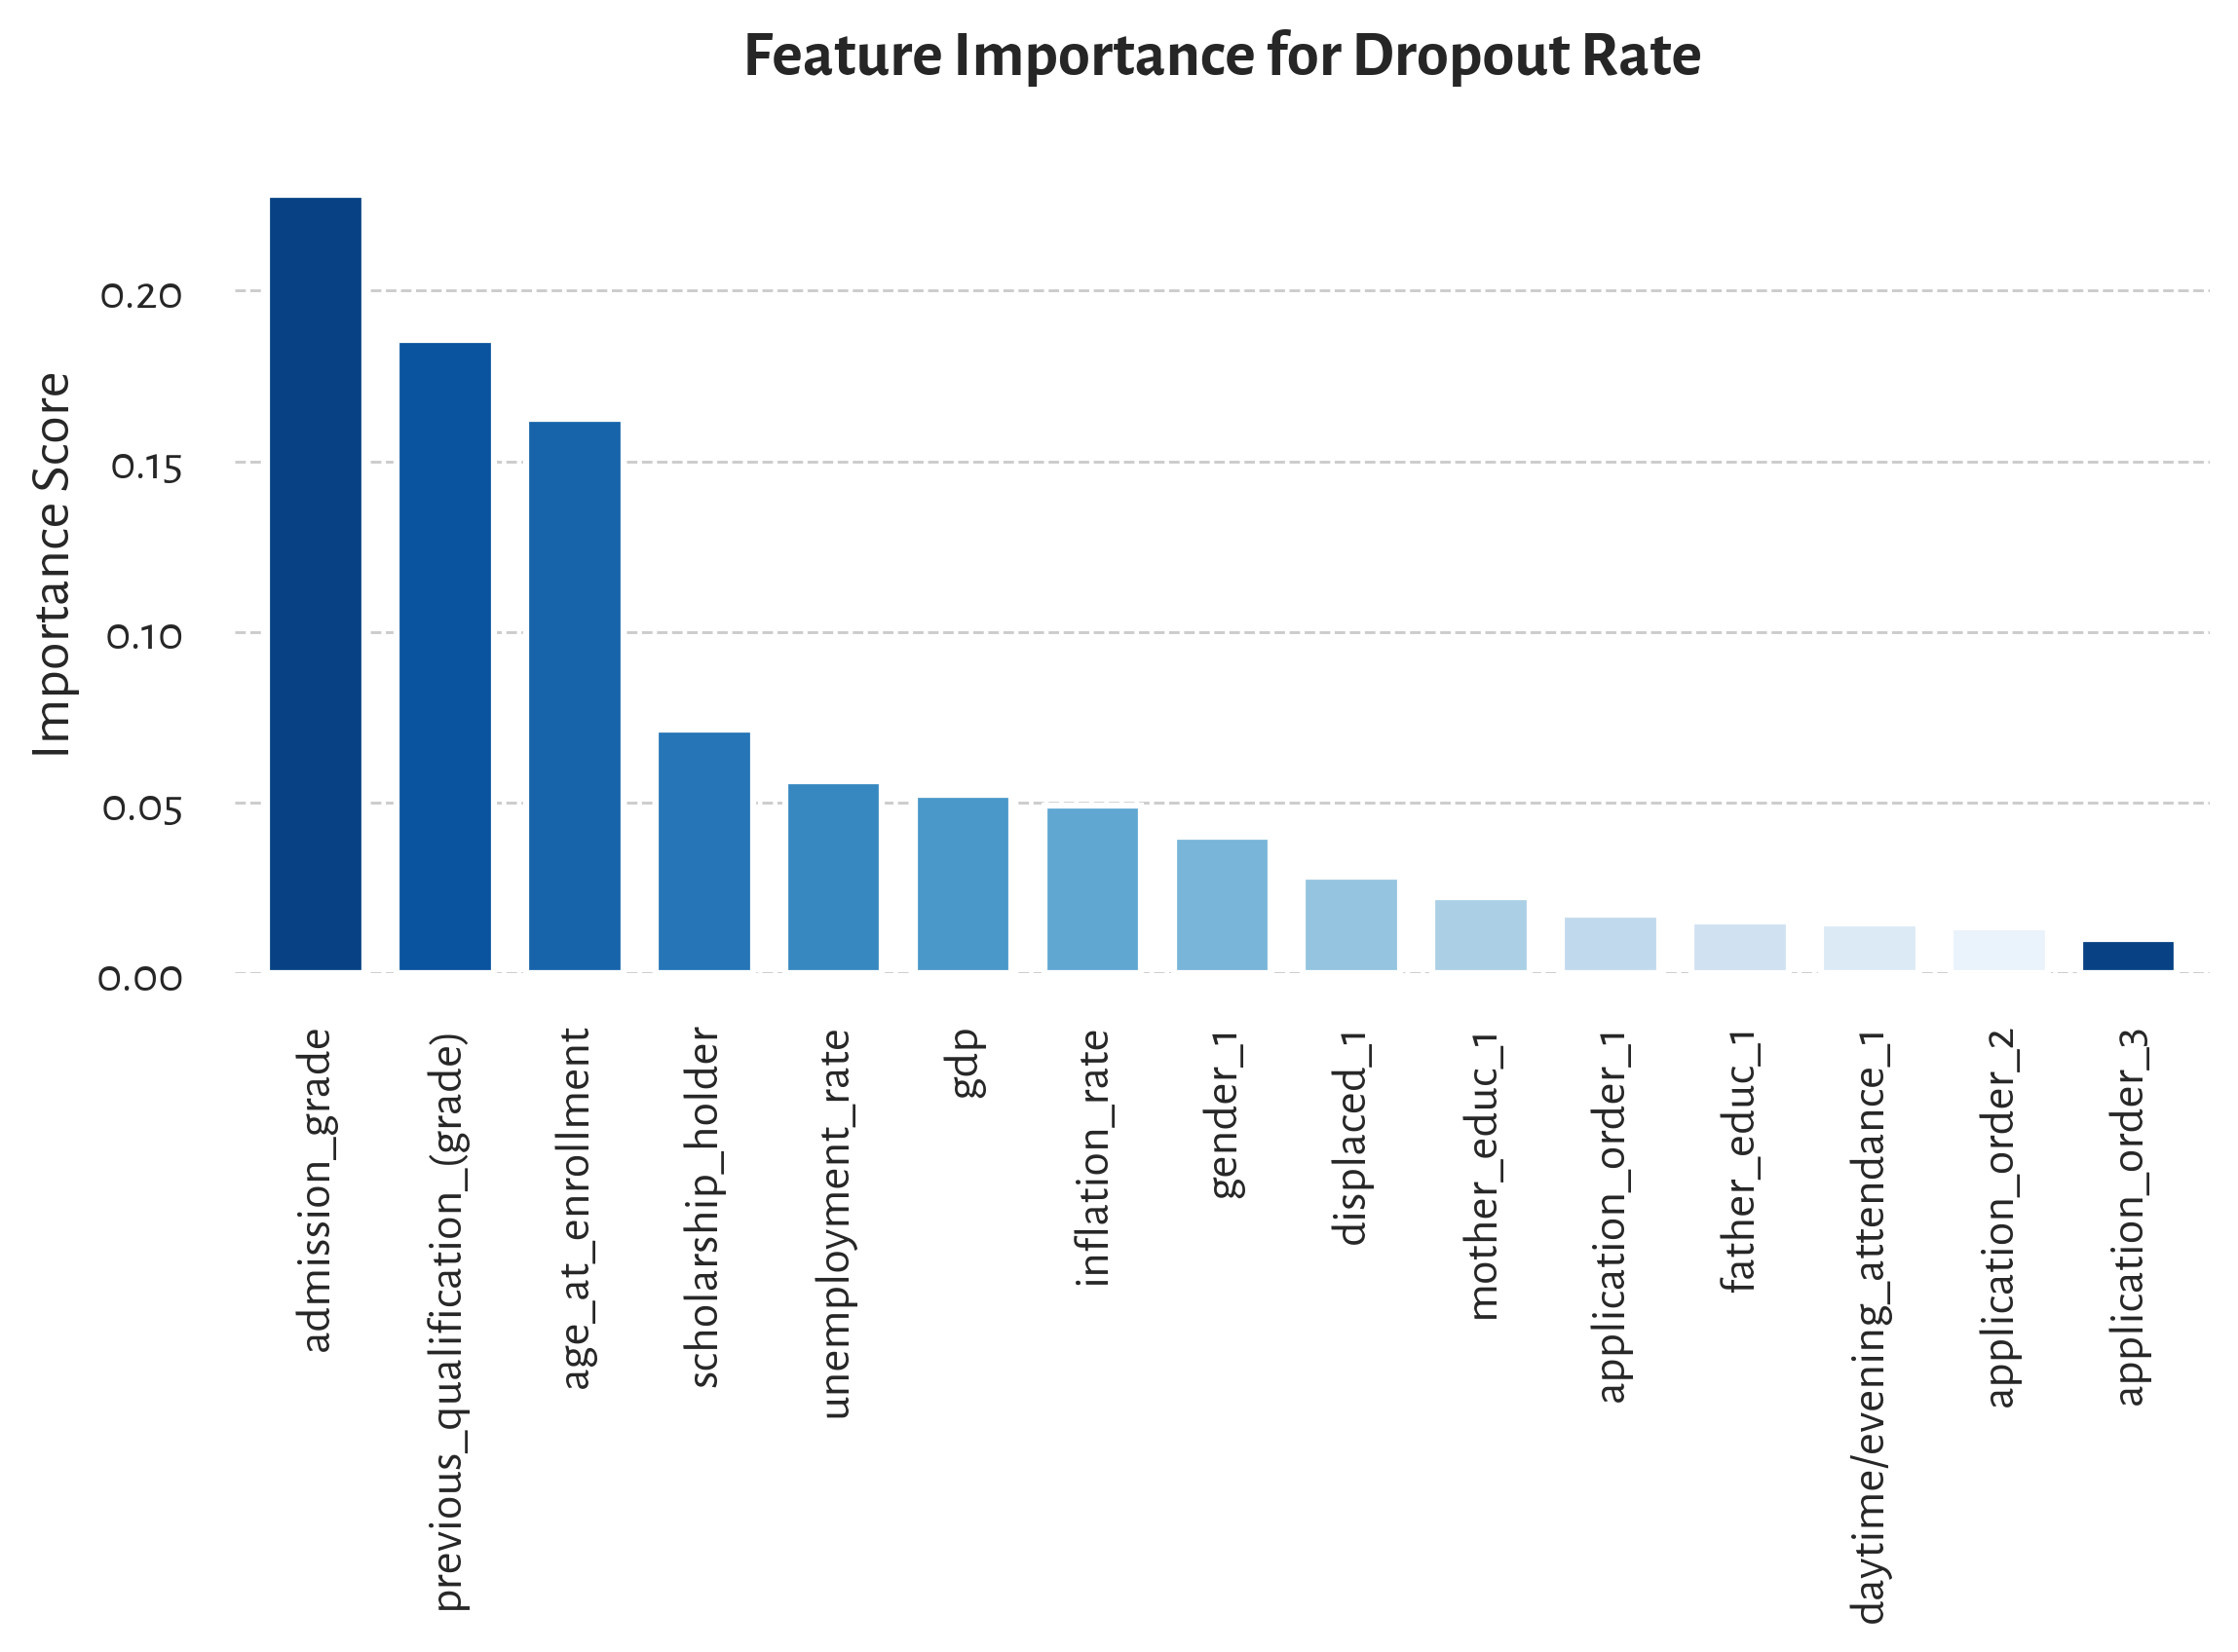
\includegraphics[width=\linewidth]{Tex_Pictures/feature_dropout}

\end{column}
\begin{column}{0.5\textwidth}
\centering
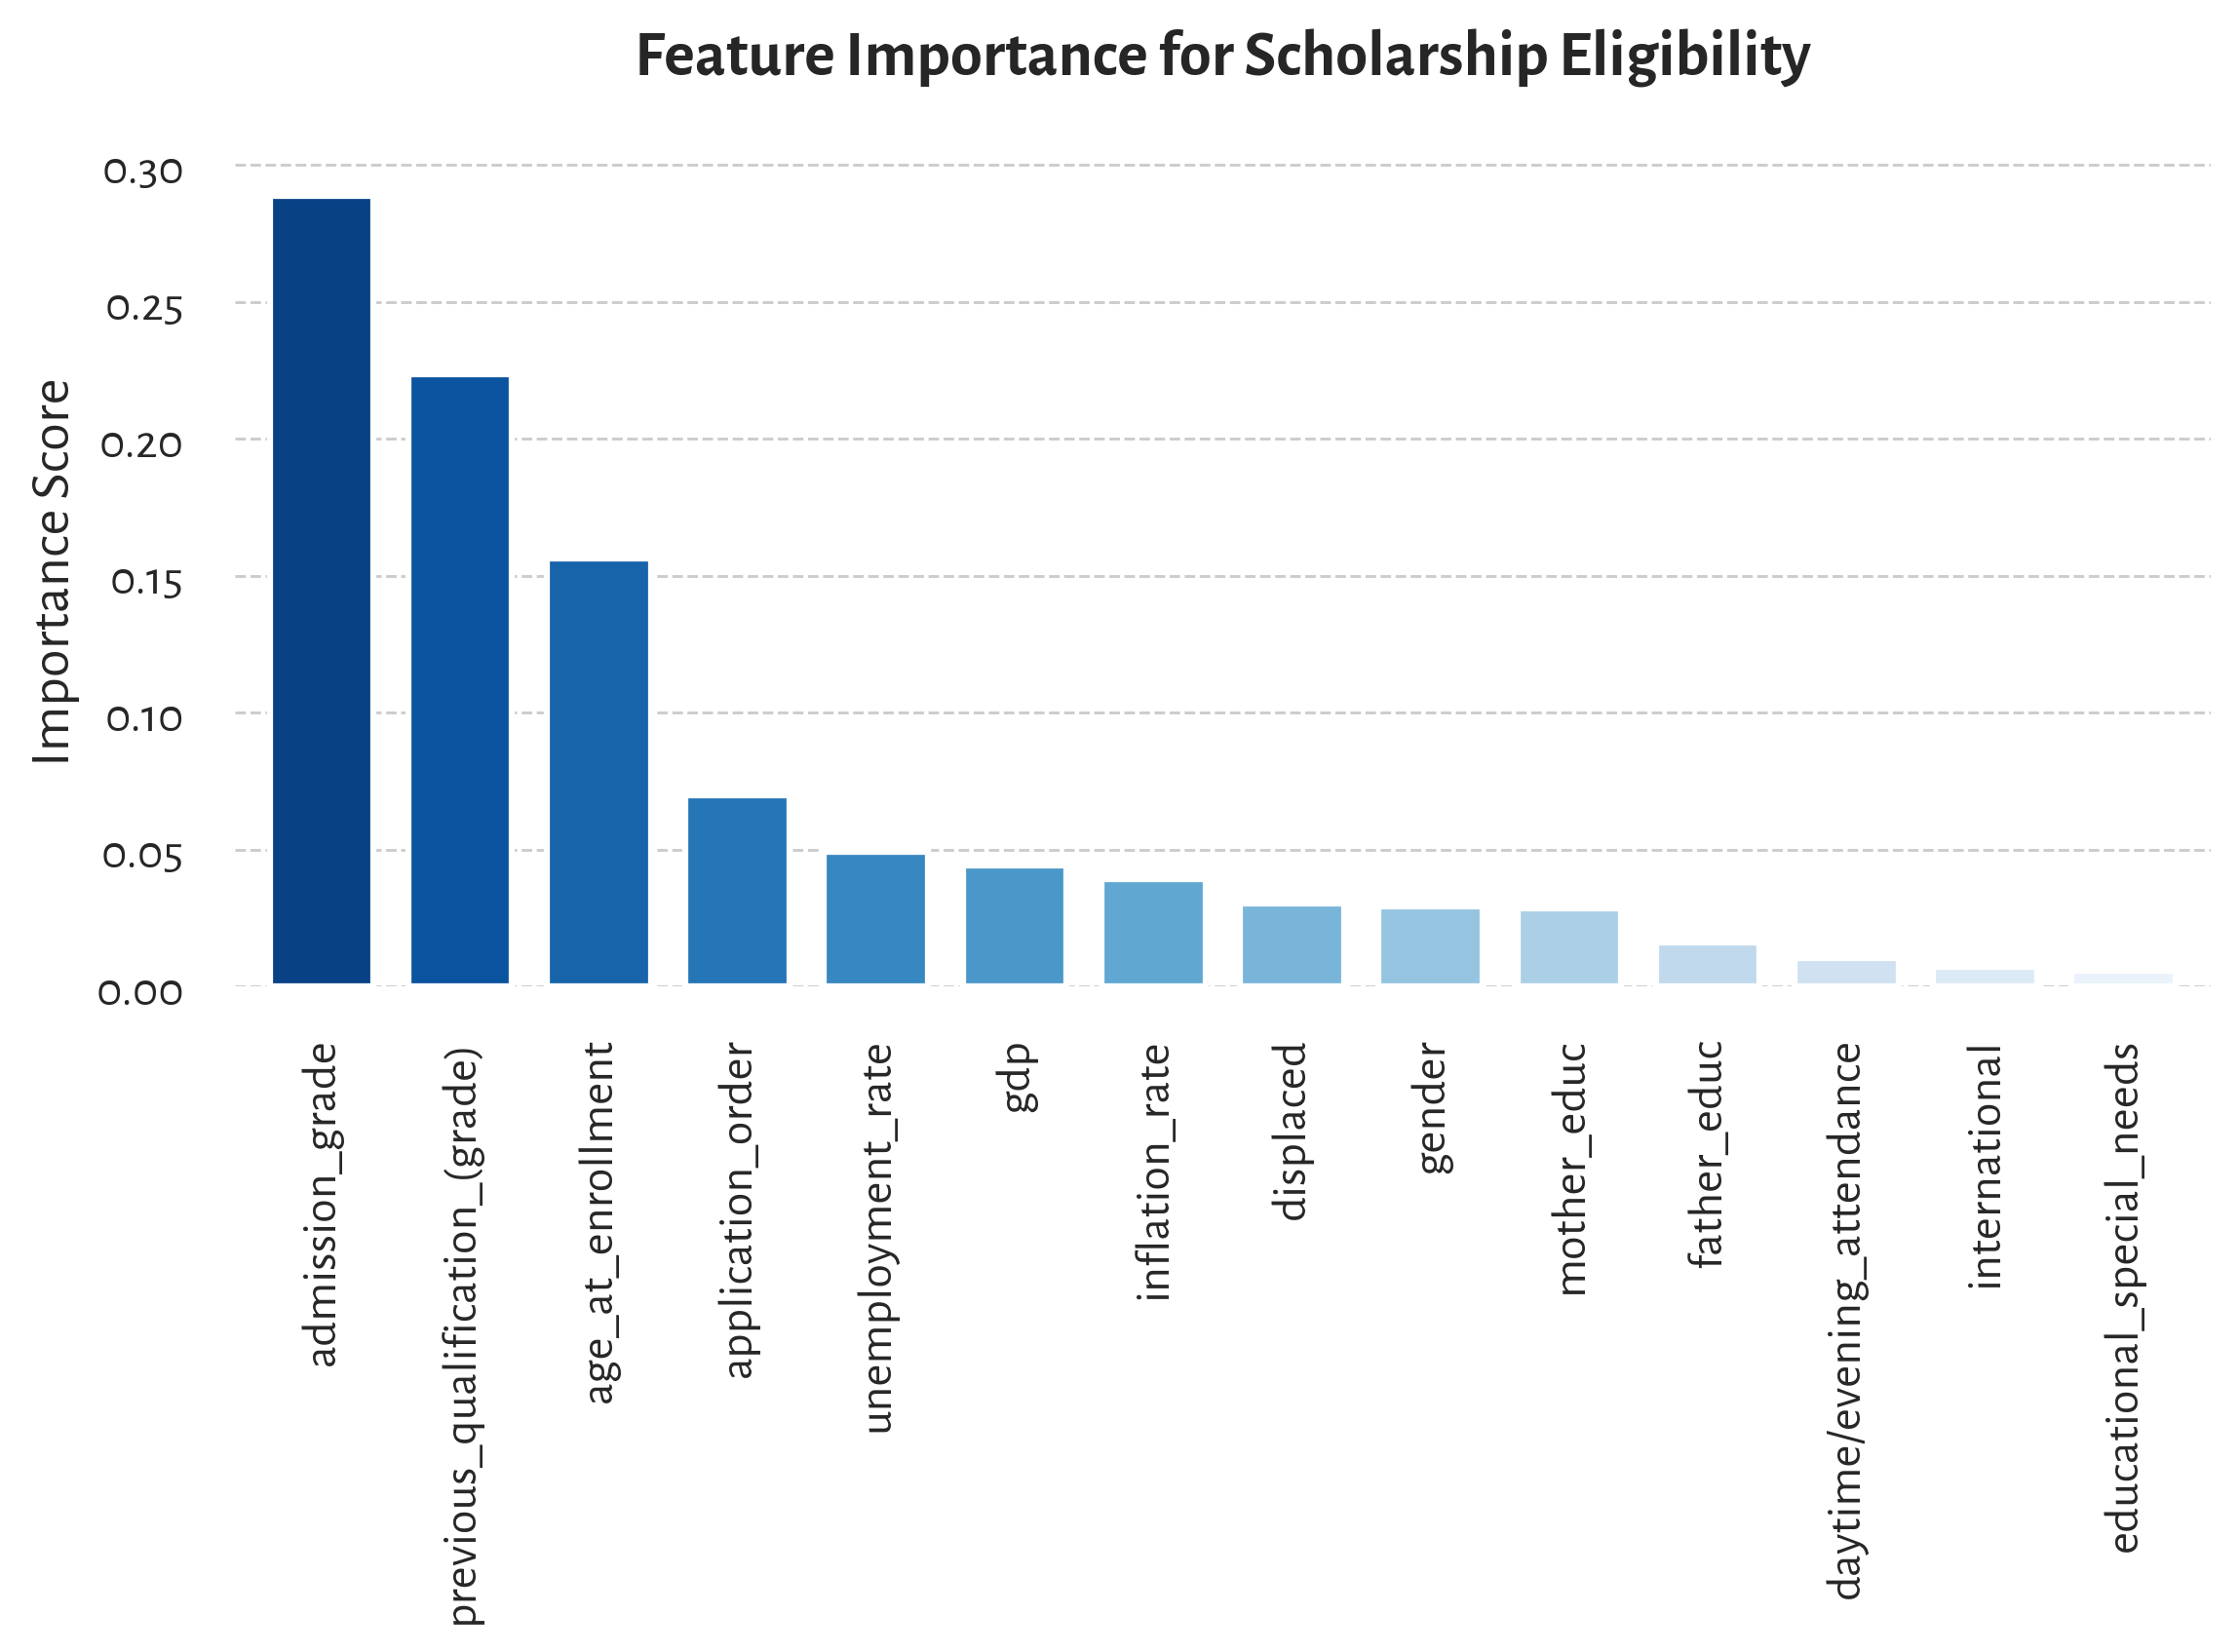
\includegraphics[width=\linewidth]{Tex_Pictures/feature_scholarship}
\end{column}
\end{columns}
\vspace{8pt}
\textbf{$\Rightarrow$ Random Forest Reveals Academic Preparation as Main Predictor of Student Outcomes} \\
\textit{our primary variables of interest - \textbf{scholarship holding} and \textbf{gender} - appear less significant.}

\end{frame}

\begin{frame}{Check 1: Identifying Key Predictors of Student Outcomes using Feature Importance}
\begin{columns}
\begin{column}{0.65\textwidth}
\vspace{10pt} \\
\textbf{Main Finding}
\begin{itemize}
	\item [$\Rightarrow$] Academic performance (e.g., \textit{admission grade}) dominates prediction, while variables like \textbf{scholarship status} and \textbf{gender} show lower importance.
\end{itemize}

\vspace{5pt}   
   
\textbf{Discussion}
\begin{itemize}[label=--, itemsep=1pt]
    \item Academic and financial variables likely influence outcomes \textit{indirectly}.
    \item Random Forest prioritizes predictive power, not causal relevance.
    \item For \textbf{direct effects}, we rely on causal models like DoubleML and DPL.
\end{itemize}


\end{column}
\begin{column}{0.35\textwidth}
\raggedright
\hspace*{-0.6cm}
\vspace*{-0.9cm}
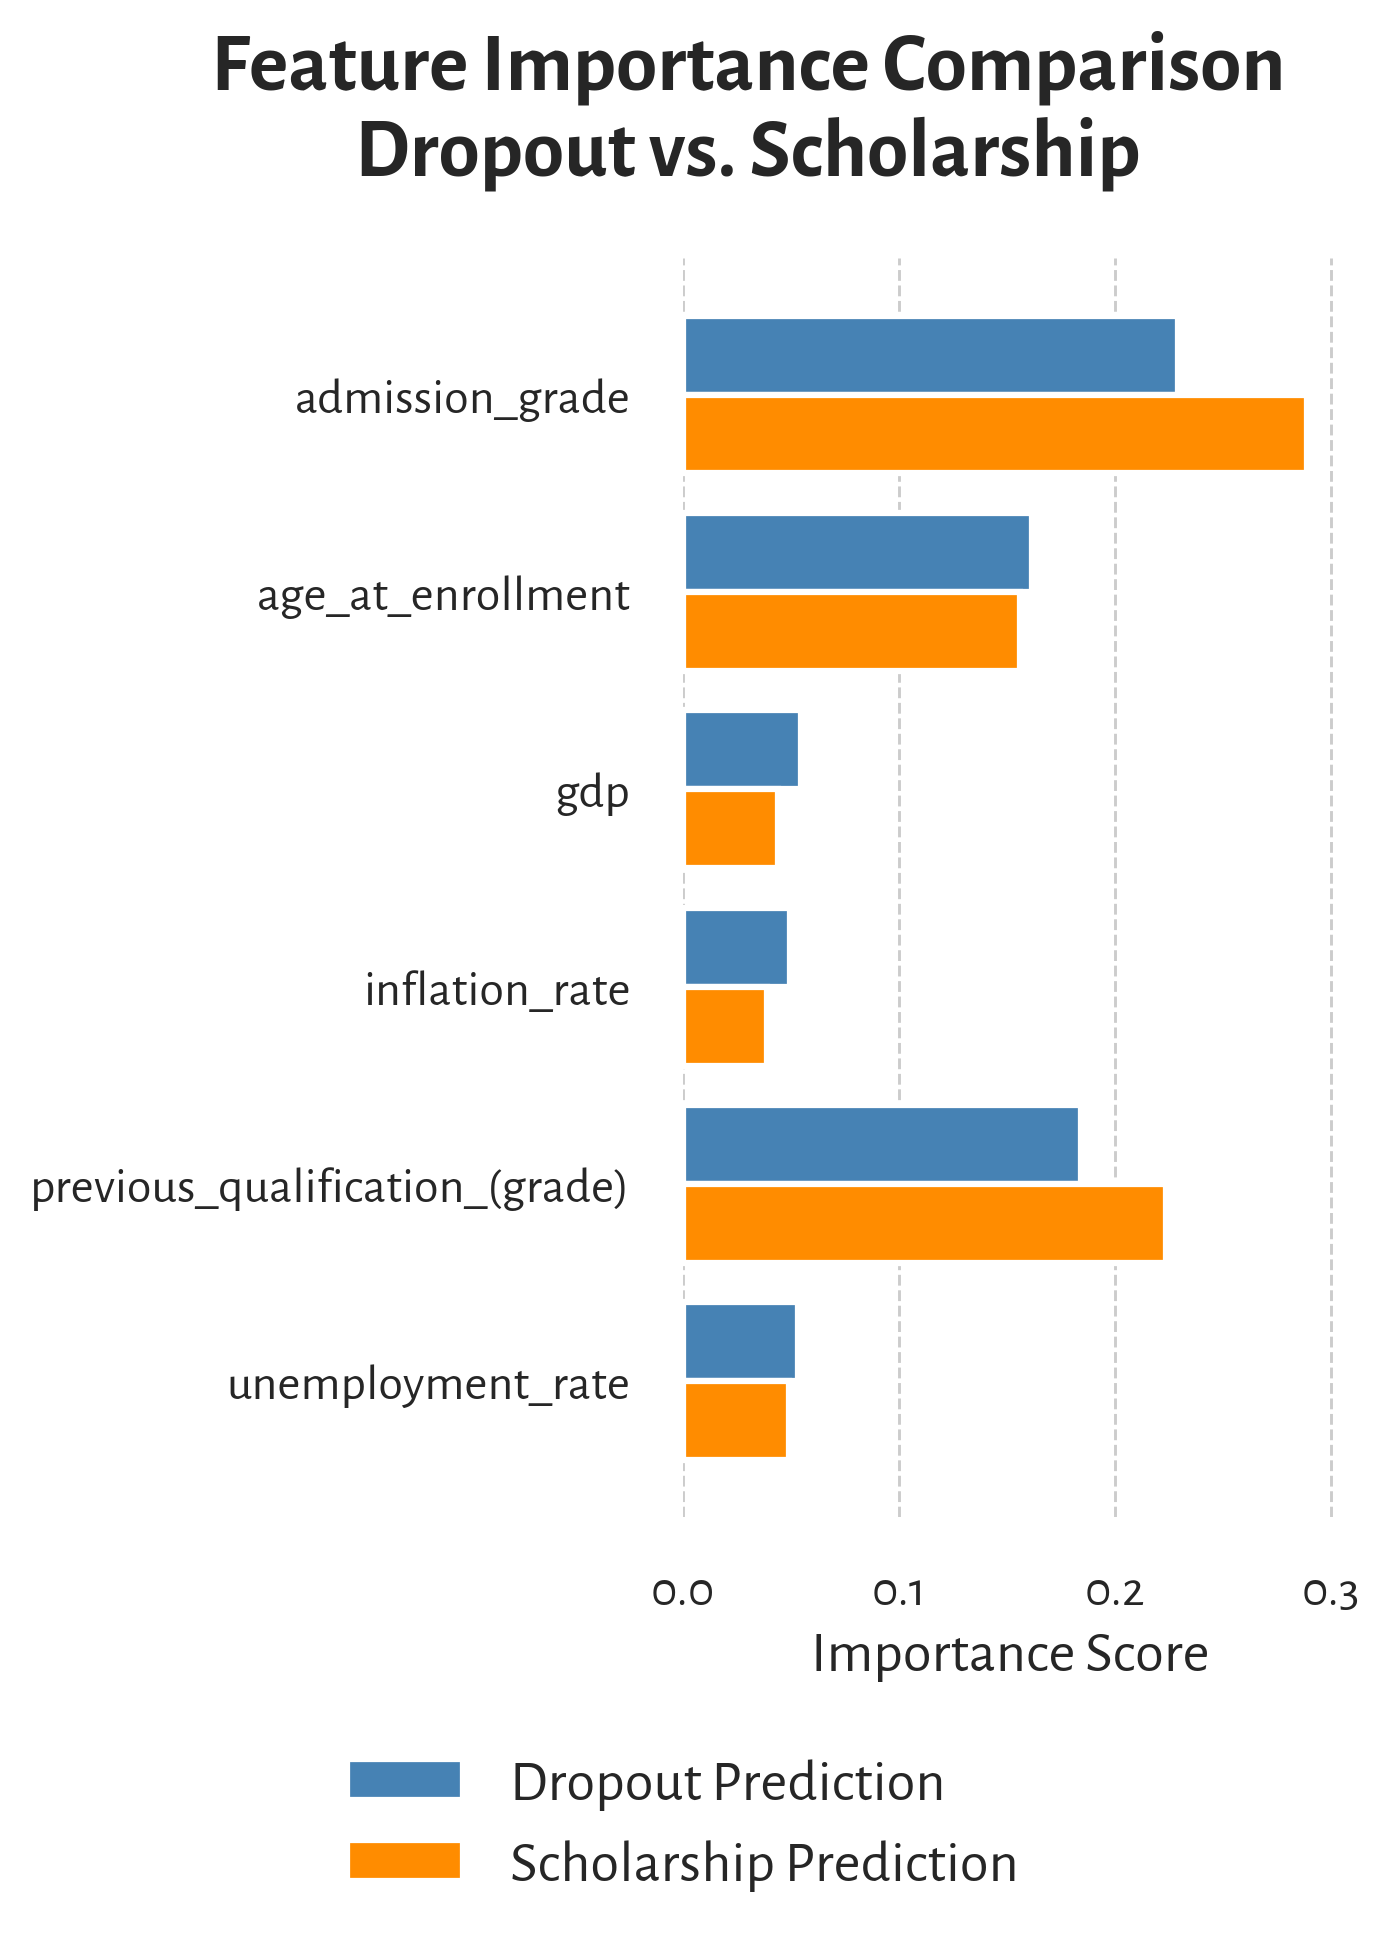
\includegraphics[width=1.05\linewidth]{Tex_Pictures/feature_importance_combined}
\end{column}
\end{columns}

\end{frame}

\begin{frame}{Check 2: Sensitivity to Covariate Selection}

\textbf{Are scholarship effects robust to different model specifications?} 

We re-estimate treatment effects using DoubleML while varying covariate sets:
\begin{itemize}[label=--, itemsep=1pt]
    \item Covariates grouped into: \textit{academic preparation, family background, economic context, and demographics.}
    \item Estimates remain statistically significant across all models for both \textbf{RQ1 (Dropout)} and \textbf{RQ2 (Graduation)}.
    \item Effects are \textbf{strongest} when controlling for \textbf{economic and parental background}.
\end{itemize}
\vspace{5pt}
\begin{block}{Conclusion}
Scholarship benefits are particularly pronounced for structurally disadvantaged students — supporting the role of financial aid in promoting equity in higher education.
\end{block}

\end{frame}


\begin{frame}{Check 2: Sensitivity to Covariate Selection: Visualizing}
\centering
\textbf{Treatment effect estimates across different covariate sets.}\\
\vspace{15pt}

\begin{columns}
\begin{column}{0.5\textwidth}
\centering
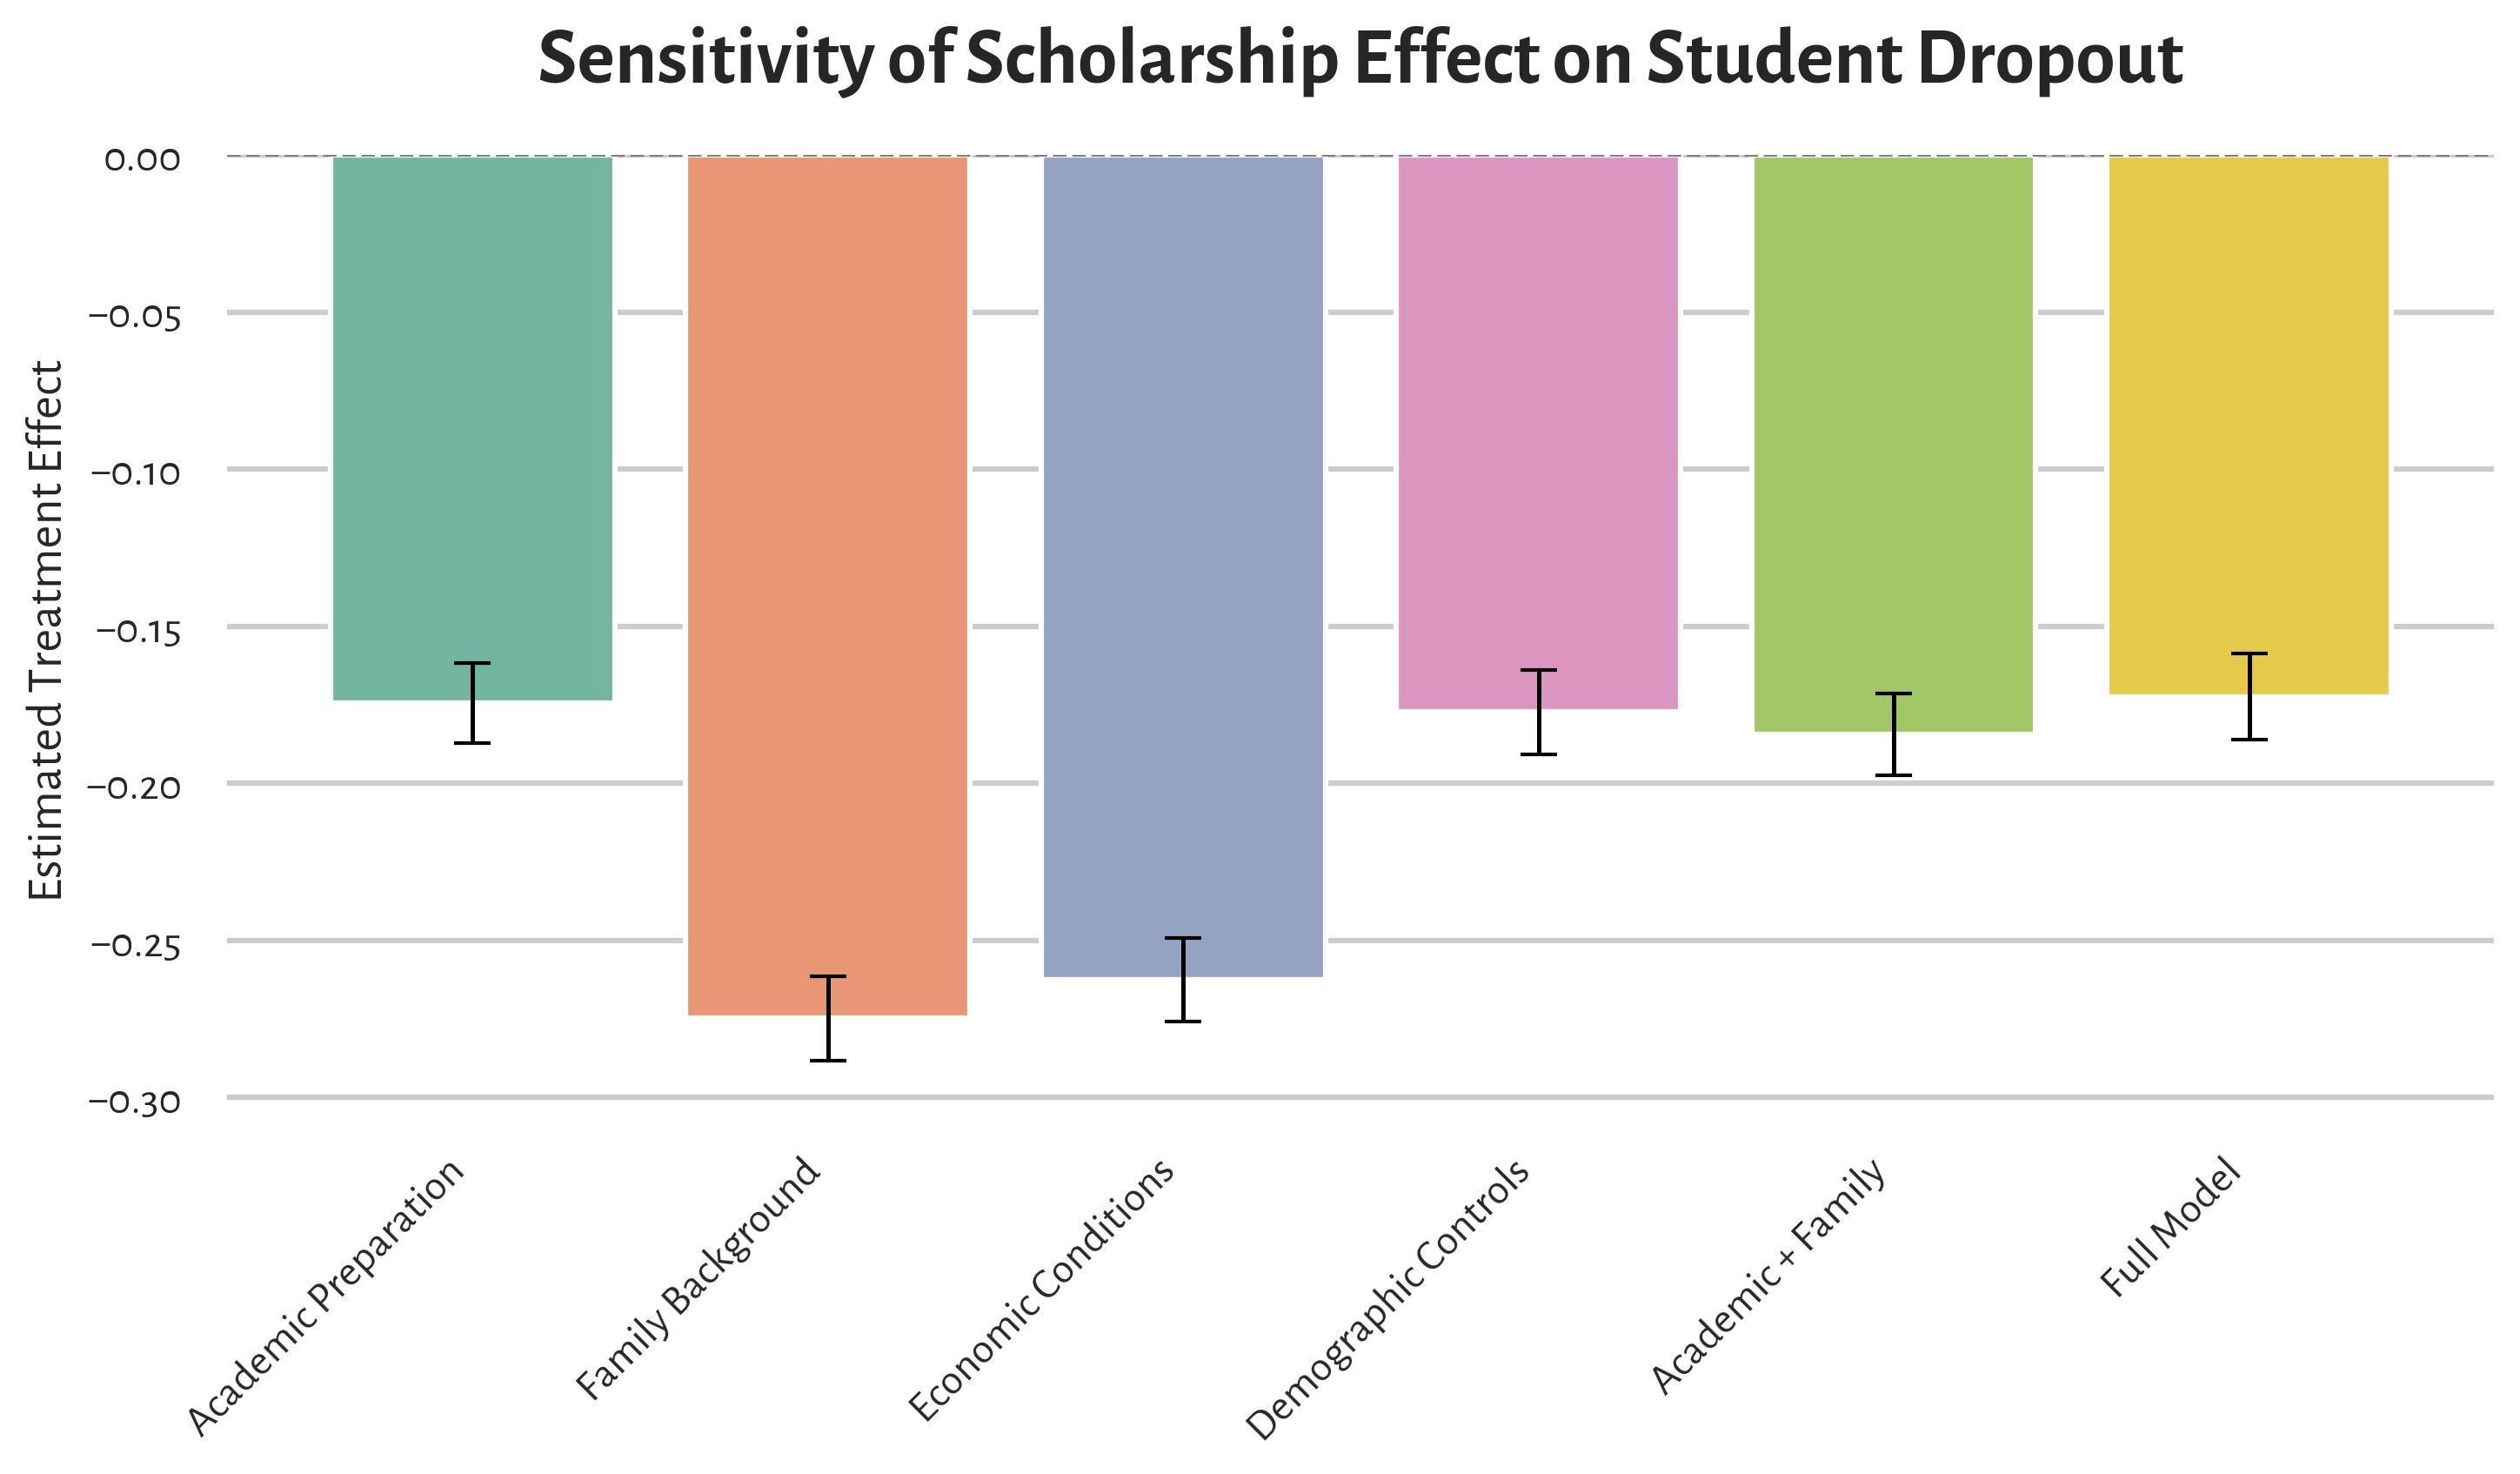
\includegraphics[width=1\linewidth]{Tex_Pictures/sensitivityrq1.png} \\
\end{column}
\begin{column}{0.5\textwidth}
\centering
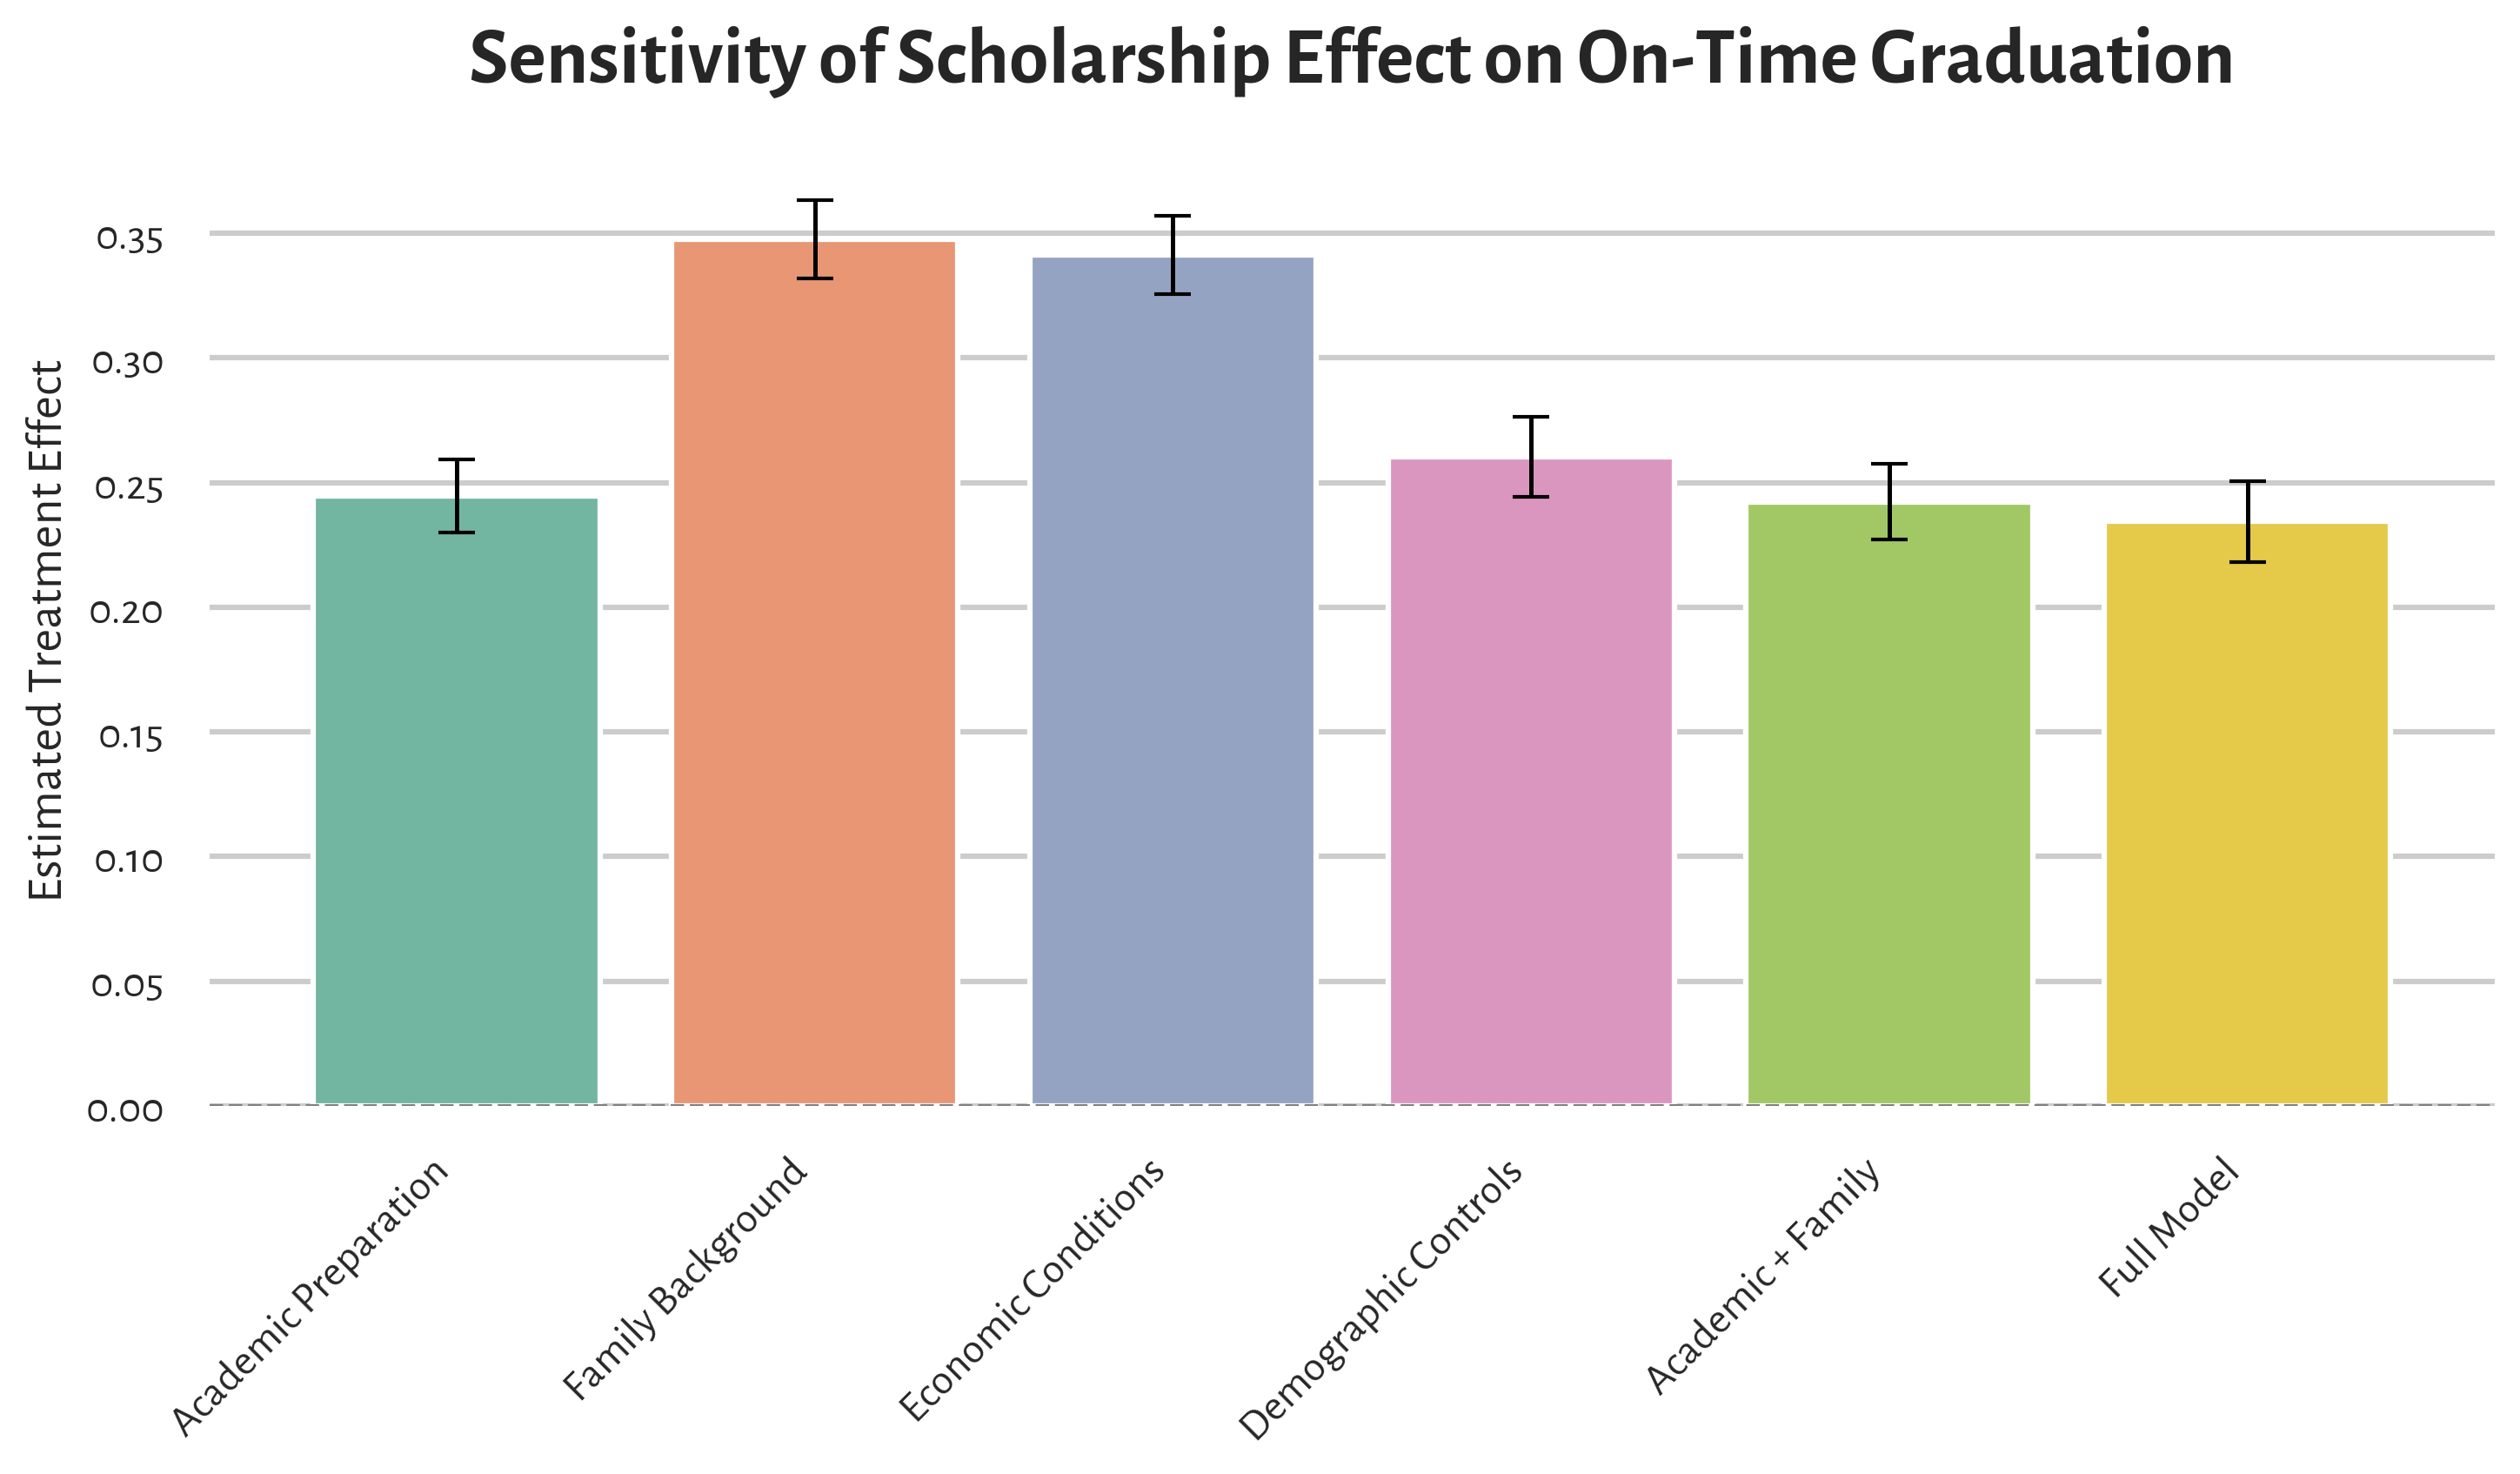
\includegraphics[width=1\linewidth]{Tex_Pictures/sensitivityrq2.png} \\
\end{column}
\end{columns}
\vspace{5pt}
$\Rightarrow$ \textbf{The direction and significance of the effect remain stable, though the magnitude varies.}\\
\textit{The strongest effects are seen when economic and family background variables are included.}
\end{frame}

\begin{frame}{Check 3: Placebo Test — Are Our Effects Spurious?}
\begin{columns}[t]

\begin{column}{0.5\textwidth}
\newline
\textbf{What if scholarships were assigned randomly?}
\begin{itemize}[label=--, itemsep=1pt]
    \item We ran a \textbf{placebo test} by randomly reassigning the scholarship variable.
    \item The fake treatment mimics the real distribution but has no connection to outcomes.
    \item We re-estimated effects using DML to check for spurious patterns.
\end{itemize}

\end{column}

\begin{column}{0.45\textwidth}
\newline
\textbf{Findings:}
\begin{itemize}[label=--, itemsep=1pt]
    \item Dropout: placebo ATE $\approx$ \textbf{+0.02}, (s.e. $\approx$ 0.015), \textit{p} $\approx$ 0.23
    \item Graduation: placebo ATE $\approx$ \textbf{–0.01}, (s.e. $\approx$ 0.017), \textit{p} $\approx$ 0.68
    \item [$\Rightarrow$] Effects are statistically insignificant and close to zero.
\end{itemize}
\end{column}
\end{columns}
\vspace{10pt}
\begin{block}{Conclusion}
The placebo test confirms that our original estimates are not driven by spurious patterns or overfitting — supporting the credibility of our causal results.
\end{block}
\end{frame}

\begin{frame}{Summary: Robustness and Sensitivity Analysis}
\textbf{Robustness Checks Support the Causal Impact of Scholarships}
\vspace{6pt}
\begin{itemize}[label=--, itemsep=3pt]
    \item Effects are \textbf{statistically significant and consistent} across model specifications.
    \item Strongest impact observed among students with \textbf{lower socio-economic background}.
    \item \textbf{Placebo test} yields no effect $\Rightarrow$ supports validity of causal claims.
\end{itemize}

\vspace{10pt}
\begin{block}{Conclusion}
Scholarships have a robust and meaningful causal impact on student outcomes — supported by multiple model checks and falsification tests.
\end{block}

\end{frame}


\section{10. Conclusion}

\begin{frame}{Conclusion: Causal Impact of Scholarships on Student Success}
	
	\textbf{Objective} 
	\vspace{-5pt}
	\begin{itemize}
	\item[$\rightarrow$]Estimate the causal effect of scholarships on dropout and graduation within 3 years 
	\item[$\rightarrow$]Data: 4,424 students from a Portuguese university (UCI dataset) 
	\end{itemize}
	\vspace{-5pt}
	
	\textbf{Methods}
	\vspace{-5pt}
	\begin{itemize}
	\item[$\rightarrow$]Double Post-Lasso: Data-driven covariate selection + OLS
	\item[$\rightarrow$]Double Machine Learning: Cross-fitting + ML models (Lasso, Random Forest)
	\end{itemize}
	\vspace{-5pt}
	
	\textbf{Main Results}
	\vspace{-5pt}
	\begin{itemize}
	\item[$\rightarrow$]Dropout $\searrow$ 17–20 \%-points; Graduation $\nearrow$ 23–28 \%-points
	\item[$\rightarrow$]Robust across estimators, regularization, covariate sets, Placebo test confirms validity
	\end{itemize}
	\vspace{-5pt}

	\textbf{Conclusion}
	\vspace{-5pt}
	\begin{itemize}
	\item[$\Rightarrow$]Scholarships causally improve student outcomes: Strong evidence for policy effectiveness.
	\item[$\Rightarrow$]Supports the expansion of financial aid as a tool to reduce dropout and boost completion.
	\end{itemize}
	
\end{frame}
  
\end{document}
























